\section{Model Development}
\subsection{Core Assumptions}

With the mathematical concepts and software tools clearly defined, a number of assumptions need to be made for the RipStik model.
\par
The RipStik can be treated as 5 separate bodies; the torsion rod (1), front plate (2), back plate (3), front caster (4), and back caster (5).

\begin{figure}[!htb]
	\centering
	\minipage{0.7\textwidth}
	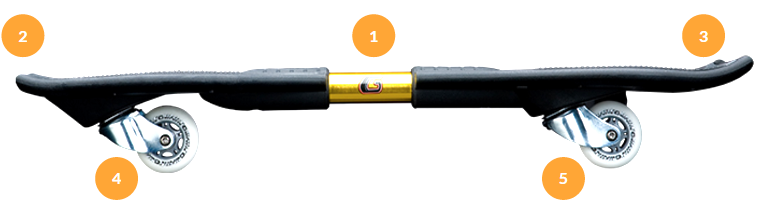
\includegraphics[width=\linewidth]{RipStikModel.png}
	\caption{Image depicting the 5 separate bodies of the RipStik}\label{fig:RipStikModel}
	\endminipage
\end{figure}  

Difficulties associated with accurately modelling the complex geometry of the RipStik lead to simplifying assumptions for the shapes of the 5 separate bodies.
The front and back plates are treated as rectangular prisms while defining inertia tensors for the bodies and the inertia tensors for the wheels are combined with the casters. 
Additionally, the casters are modelled as skates to emulate the non-slip behaviour of the wheels without consideration for the rolling dynamics. 
The rolling dynamics of the wheels are determined to be inconsequential to the modelling process for the purpose of developing a control system.
\par
The spring in the torsion rod is omitted in modelling considerations as it serves only to aid in rider comfort, and as such is not a critical component of the RipStik's dynamics. 
Including the rod will add unnecessary complexity to the system in the form of kinetic energy.
Friction between the bodies of the RipStik is omitted as it is difficult to accurately model and has negligible impact on the general dynamics of the system.

\subsection{Coordinate Systems}

The initial focus for developing a mathematical model of the RipStik is determining the number of degrees of freedom in the system. 
A coordinate system is defined, assumptions are made, and Euler angles are applied to said coordinate system so that all degrees of freedom can be explicitly defined.
\par
A body-fixed coordinate system for the RipStik is developed with the origin was placed at the centre of the torsion bar. 
The $x$-$y$ plane is located parallel to the RipStik plates at rest with no torsion applied.
The $+x$ direction points through the torsion bar towards the front plate. The $z$ axis is normal to the $x$-$y$ plane, with $+z$ pointing upwards. The $+y$ direction is defined based on the right hand rule.
With the coordinate system defined, Euler angles are implemented to represent the roll ($\alpha$), pitch ($\psi$), and yaw ($\theta$) of the system. These are rotations about the $x$, $y$, and $z$ axes respectively.
The coordinate system with $x$,$y$,$z$, $\alpha$, $\psi$, and $\theta$ is defined as shown in Figure \ref{fig:RipStikCoord}.
\begin{figure}[!htb]
	\centering
	\minipage{0.5\textwidth}
	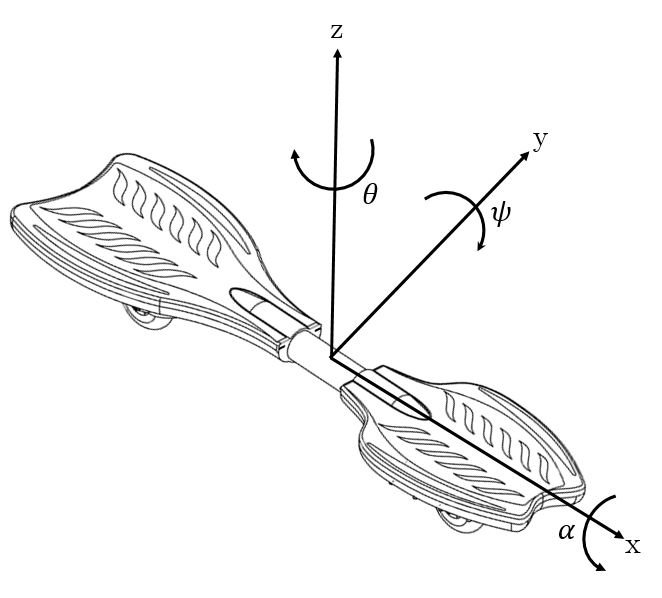
\includegraphics[width=\linewidth]{DOFpart1.jpg}
	\caption{Degrees of freedom $x$,$y$,$z$, $\alpha$, $\psi$, and $\theta$ for the RipStik}\label{fig:RipStikCoord}
	\endminipage
\end{figure}

The roll angles ($\alpha$) describe the rotation of the deck platforms about the $x$-axis. There are two roll angles corresponding to the RipStik; one for the front platform ($\alpha_{fp}$) and the second for the rear platform ($\alpha_{bp}$).
\begin{figure}[!htb]
	\centering
	\minipage{0.5\textwidth}
	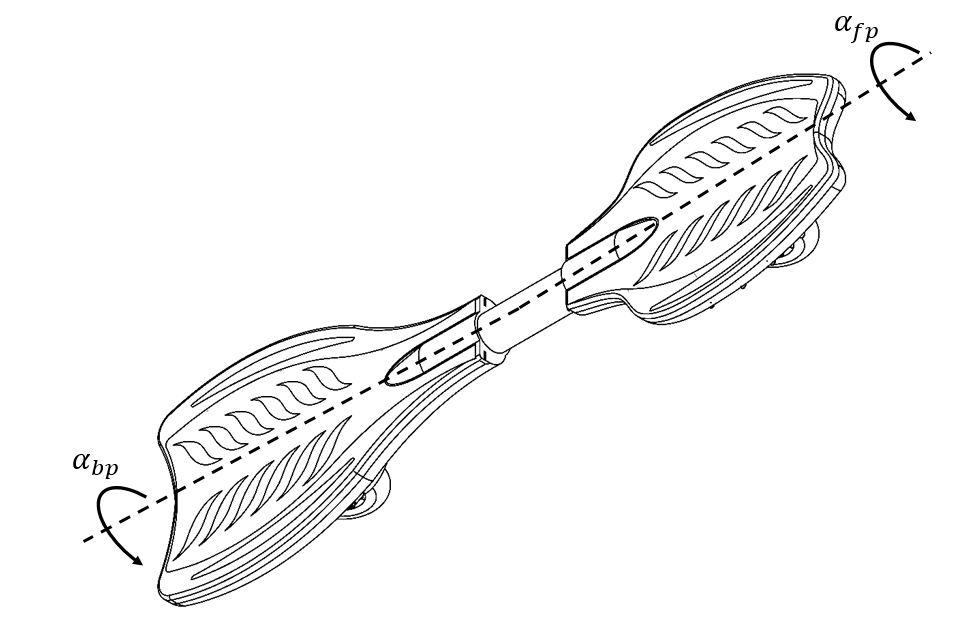
\includegraphics[width=\linewidth]{DOFpart2.jpg}
	\caption{Degrees of freedom for the roll of the front plate ($\alpha_{fp}$) and back plate ($\alpha_{bp}$) on the RipStik}\label{fig:RipStikroll}
	\endminipage
\end{figure}

The yaw angle ($\theta$) is the angle of the system about the $z$-axis (right hand rule applied). There are two yaw angles corresponding to the RipStik; one for the front caster ($\theta_{fc}$), and the second for the back caster ($\theta_{bc}$). The wheels are completely unbounded in their ability to rotate, and can pivot through [0, 2$\pi$].
\begin{figure}[!htb]
	\centering
	\minipage{0.5\textwidth}
	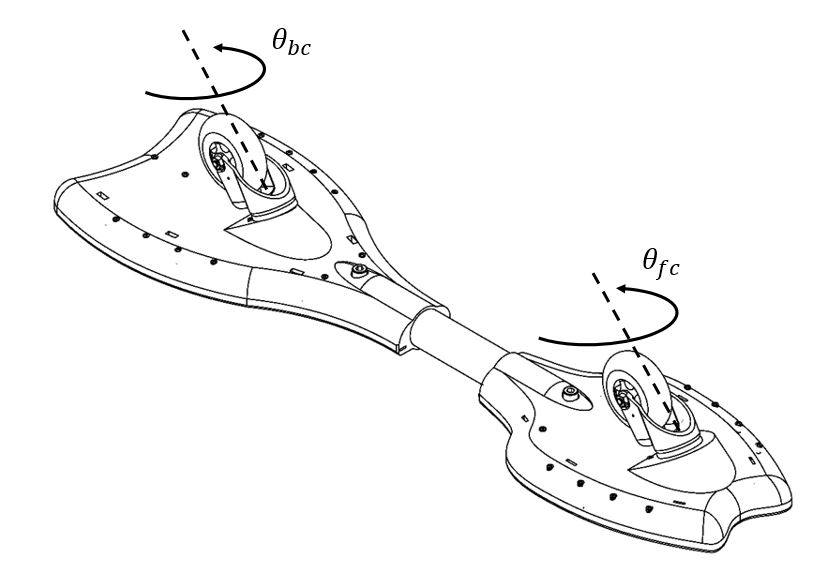
\includegraphics[width=\linewidth]{DOFpart3.jpg}
	\caption{Degrees of freedom for the yaw of the front caster ($\theta_{fc}$) and back caster ($\theta_{bc}$) on the RipStik }\label{fig:RipStikyaw}
	\endminipage
\end{figure}
The RipStik has ten degrees of freedom represented by [$x$, $y$, $z$, $\alpha$, $\psi$, $\theta$, $\alpha_{fp}$, $\alpha_{bp}$, $\theta_{fc}$, $\theta_{bc}$].
Position vectors are then constructed to define the position of each body in the RipStik relative to the others, connecting them back to the global position $(x,y,z)$.
\subsubsection{Test Case - Caster Rotation}

In order to validate the selected coordinate system, a test case is conducted for the RipStik. This is done by analyzing the behaviour of the caster as it completes a full revolution (2$\pi$ radians).
The output for the $x$ ,$y$, and $z$ positions of the contact point at the bottom of the caster is plotted as a function of the casters rotation, as shown in Figure \ref{fig:CasterWheel2DTest}.

\begin{figure}[!htb]
	\centering
	\minipage{0.7\textwidth}
	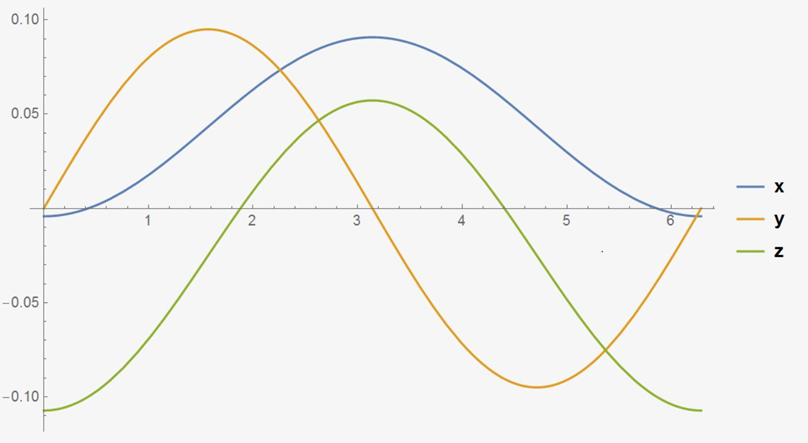
\includegraphics[width=\linewidth]{CasterWheel2DTest.png}
	\caption{The $x$ ,$y$, and $z$ positions of the caster were plotted as a function of the caster angle (in radians)}\label{fig:CasterWheel2DTest}
	\endminipage
\end{figure} 

In addition to the two-dimensional plot, a three-dimensional plot is generated to verify that the casters' behaviour aligned with expectations based on experimentation with a physical RipStik. The three-dimensional plot is shown in Figure \ref{fig:CasterWheel3DTest}.

\begin{figure}[!htb]
	\centering
	\minipage{0.7\textwidth}
	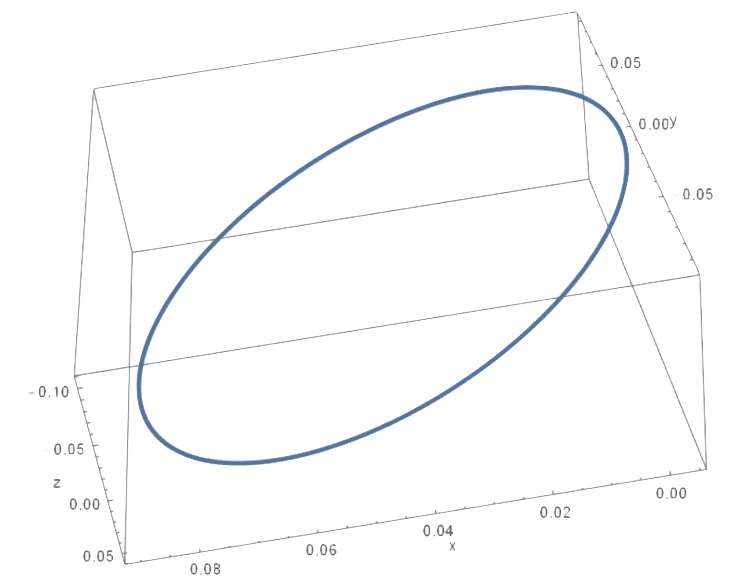
\includegraphics[width=\linewidth]{CasterWheel3DTest.png}
	\caption{The X ,Y, and Z positions of the caster were plotted as a function of the caster angle (in radians) on a three-dimensional plot}\label{fig:CasterWheel3DTest}
	\endminipage
\end{figure} 

\subsubsection{Model Implementation}

With the test case completed and verified, the coordinate system for the RipStik model can be verified for each degree of freedom in the system in the same manner as the caster unit test. 
This is completed by applying the output from Mathematica into the ThreeJS based visualization tool.
\subsubsection{Validation}
Each degree of freedom in the system behaved as expected. 
This demonstrates that the position vectors and rotation matrices are properly defined, meaning the equations of motion can be developed.
\subsection{Equations of Motion}

In order to develop the equations of motion for the RipStik, the Lagrangian needs to be explicitly developed. Given Equation \ref{eq:Lagrange}, it is necessary to break down the components of kinetic and potential energies in the system.

The kinetic energy in the system is composed of translational and rotational components.
The Translational Kinetic Energy (TKE) is modeled in the following fashion:

\begin{equation}
\label{eq:TKE}
\text{TKE} = \frac{1}{2}{\text{m}}{\lvert \lvert {\dot{\text{r}}^2} \rvert \rvert}
\end{equation}

In Equation \ref{eq:TKE}, $m$ represents the mass of the body and $\dot{r}$ represents the translational velocity of the body.
\par
The Rotational kinetic energy (RKE) is modelled in the following fashion:

\begin{equation}
\label{eq:RKE}
\text{RKE} = \frac{1}{2}({\text{I}}{\omega(t)})^T\omega(t)
\end{equation}

In Equation \ref{eq:RKE}, $I$ represents the inertia tensor of the body, and $\omega(t)$ represents the angular velocity of the body.

Solving for the angular velocity of the body requires the following process. First, $\hat{\omega(t)}$ is solved for using Equation \ref{eq:omegahat}.

\begin{equation}
\label{eq:omegahat}
\hat{\omega}(t)=R^T(t)\dot{R(t)}
\end{equation}

Equation \ref{eq:omegahat} generates a $3x3$ skew-symmetric matrix. The angular velocity is then a column vector composed of 3 elements from $\hat{\omega}(t)$, as seen in Equation \ref{eq:omega}.

\begin{equation}
\label{eq:omega}
\omega(t)=\begin{bmatrix}
\hat{\omega}(t)[3,2] \\
\hat{\omega}(t)[1,3] \\
\hat{\omega}(t)[2,1]\\
\end{bmatrix}
\end{equation}

The potential energy in the system is composed of only Gravitational Potential Energy (GPE). This is modelled by Equation \ref{eq:GPE}.

\begin{equation}
\label{eq:GPE}
\text{GPE} = {\text{m}}{\text{g}}{\text{h}}
\end{equation}

In Equation \ref{eq:GPE}, $m$ represents the mass of the body and $h$ represents the height of the body relative to the ground plane.

With the kinetic and potential energies explicitly defined, the Lagrangian can be written as follows:

\begin{equation}
L= \frac{1}{2}{\text{m}}{\lvert \lvert {\dot{\text{r}}^2} \rvert \rvert} + \frac{1}{2}({\text{I}}{\omega(t)})^T\omega(t) - {\text{m}}{\text{g}}{\text{h}}
\end{equation}

The explicit Lagrangian can then be applied to the Euler-Lagrange equations to develop the ten unconstrained equations of motion for each degree of freedom using Equation \ref{eq:UEOM}.

\subsubsection{Test Case - Uncontrolled Inverted Pendulum}\label{sec:testcaseip}

The equations of motion were validated using an unconstrained system. A pendulum attached to a moving cart, with an initial position pointing upwards, was modelled using Lagrangian mechanics. 
The mass of the cart is defined as $m_{1}$ and the mass of the pendulum is defined as $m_{2}$. 
The coordinate system can be seen in figure \ref{fig:pendulumcart}.

\begin{figure}[!htb]
	\centering
	\minipage{0.5\textwidth}
	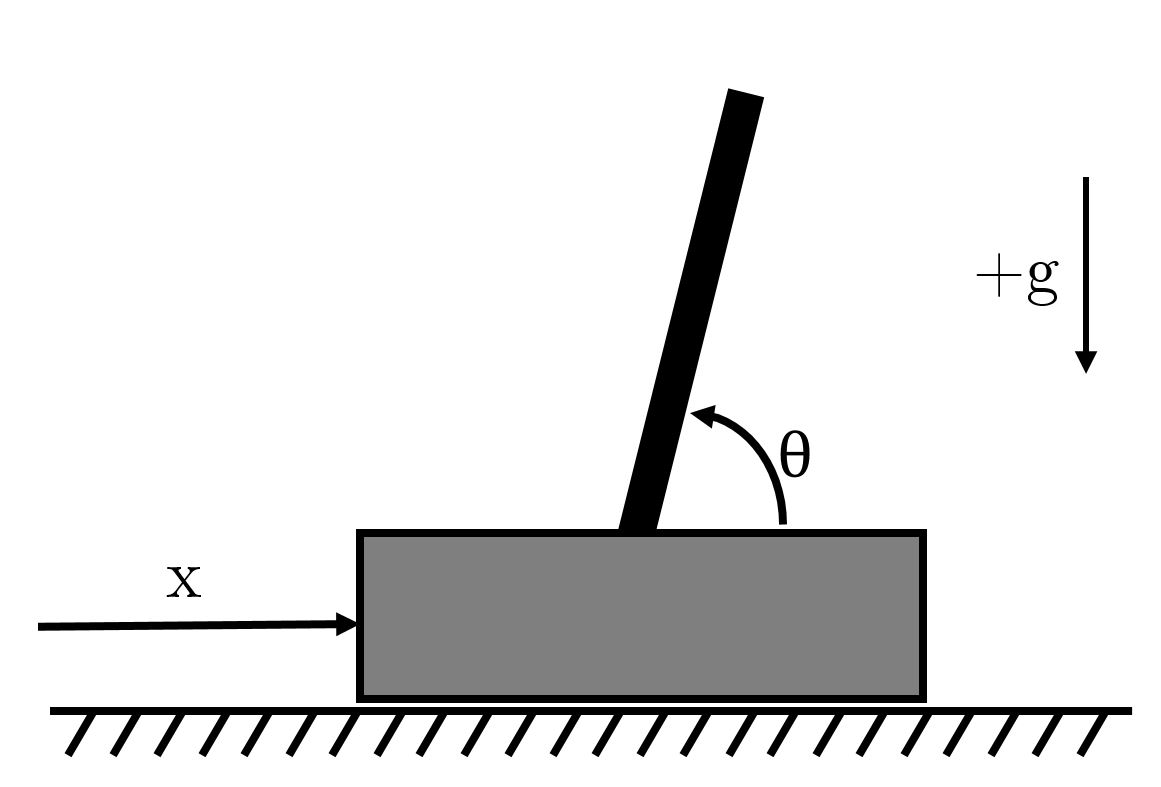
\includegraphics[width=\linewidth]{pendulumcart}
	\caption{Model set-up for the pendulum cart example}\label{fig:pendulumcart}
	\endminipage
\end{figure} 

The Lagrangian for the system is seen in Equation \ref{eq:CartLagrange}.

\begin{equation}
\label{eq:CartLagrange}
L = \frac{1}{2}m_{1}X'(t)^2+\frac{1}{2}m_{2}(2gL\sin\theta(t)+2L^2\theta'(t)^2-2L\sin\theta(t)\theta'(t)X'(t)+X'(t)^2) 
\end{equation}

With the Lagrangian developed, the equations of motion were solved for the two degrees of freedom (X(t), $\theta(t)$):

\begin{equation}
Lm_{2}\cos\theta(t)\theta'(t)^2+Lm_{2}\sin\theta(t)\theta''(t)-(m_{1}+m_{2})X''(t) = 0
\end{equation}

\begin{equation}
Lm_{2}(g\cos\theta(t)-2L\theta''(t)+\sin\theta(t)X''(t)) = 0
\end{equation}

With these equations of motion, it was confirmed that the pendulum reacts as expected to the motion of the cart.

\subsubsection{Model Implementation}

With the test case complete, the equations of motion can be tested on the RipStik model. The $z$ coordinate in the centre of the torsion rod of the RipStik is fixed.
An initial roll angle of $\frac{\pi}{4}$ is applied to the front plate ($\alpha_{fp}$), and an initial roll angle of $-\frac{\pi}{4}$ is applied to the back plate ($\alpha_{bp}$). 

\subsubsection{Validation}

When the model implementation is tested with the conditions specified previously, the RipStik behaves as expected. 
The front and back plates experience an oscillating motion between $\frac{\pi}{4}$ and $-\frac{\pi}{4}$ degrees, with the casters rotating between $\frac{\pi}{4}$ and $-\frac{\pi}{4}$ degrees. 
Plots for roll of the front plate ($\alpha_{fp}$), roll of the back plate ($\alpha_{bp}$), yaw of the front caster ($\theta_{fc}$), and yaw of the back caster ($\theta_{bc}$) are plotted to ensure that the motion of the Ripstik aligns with the expected behaviour.

\begin{figure}[!htb]
	\centering
	\minipage{0.4\textwidth}
	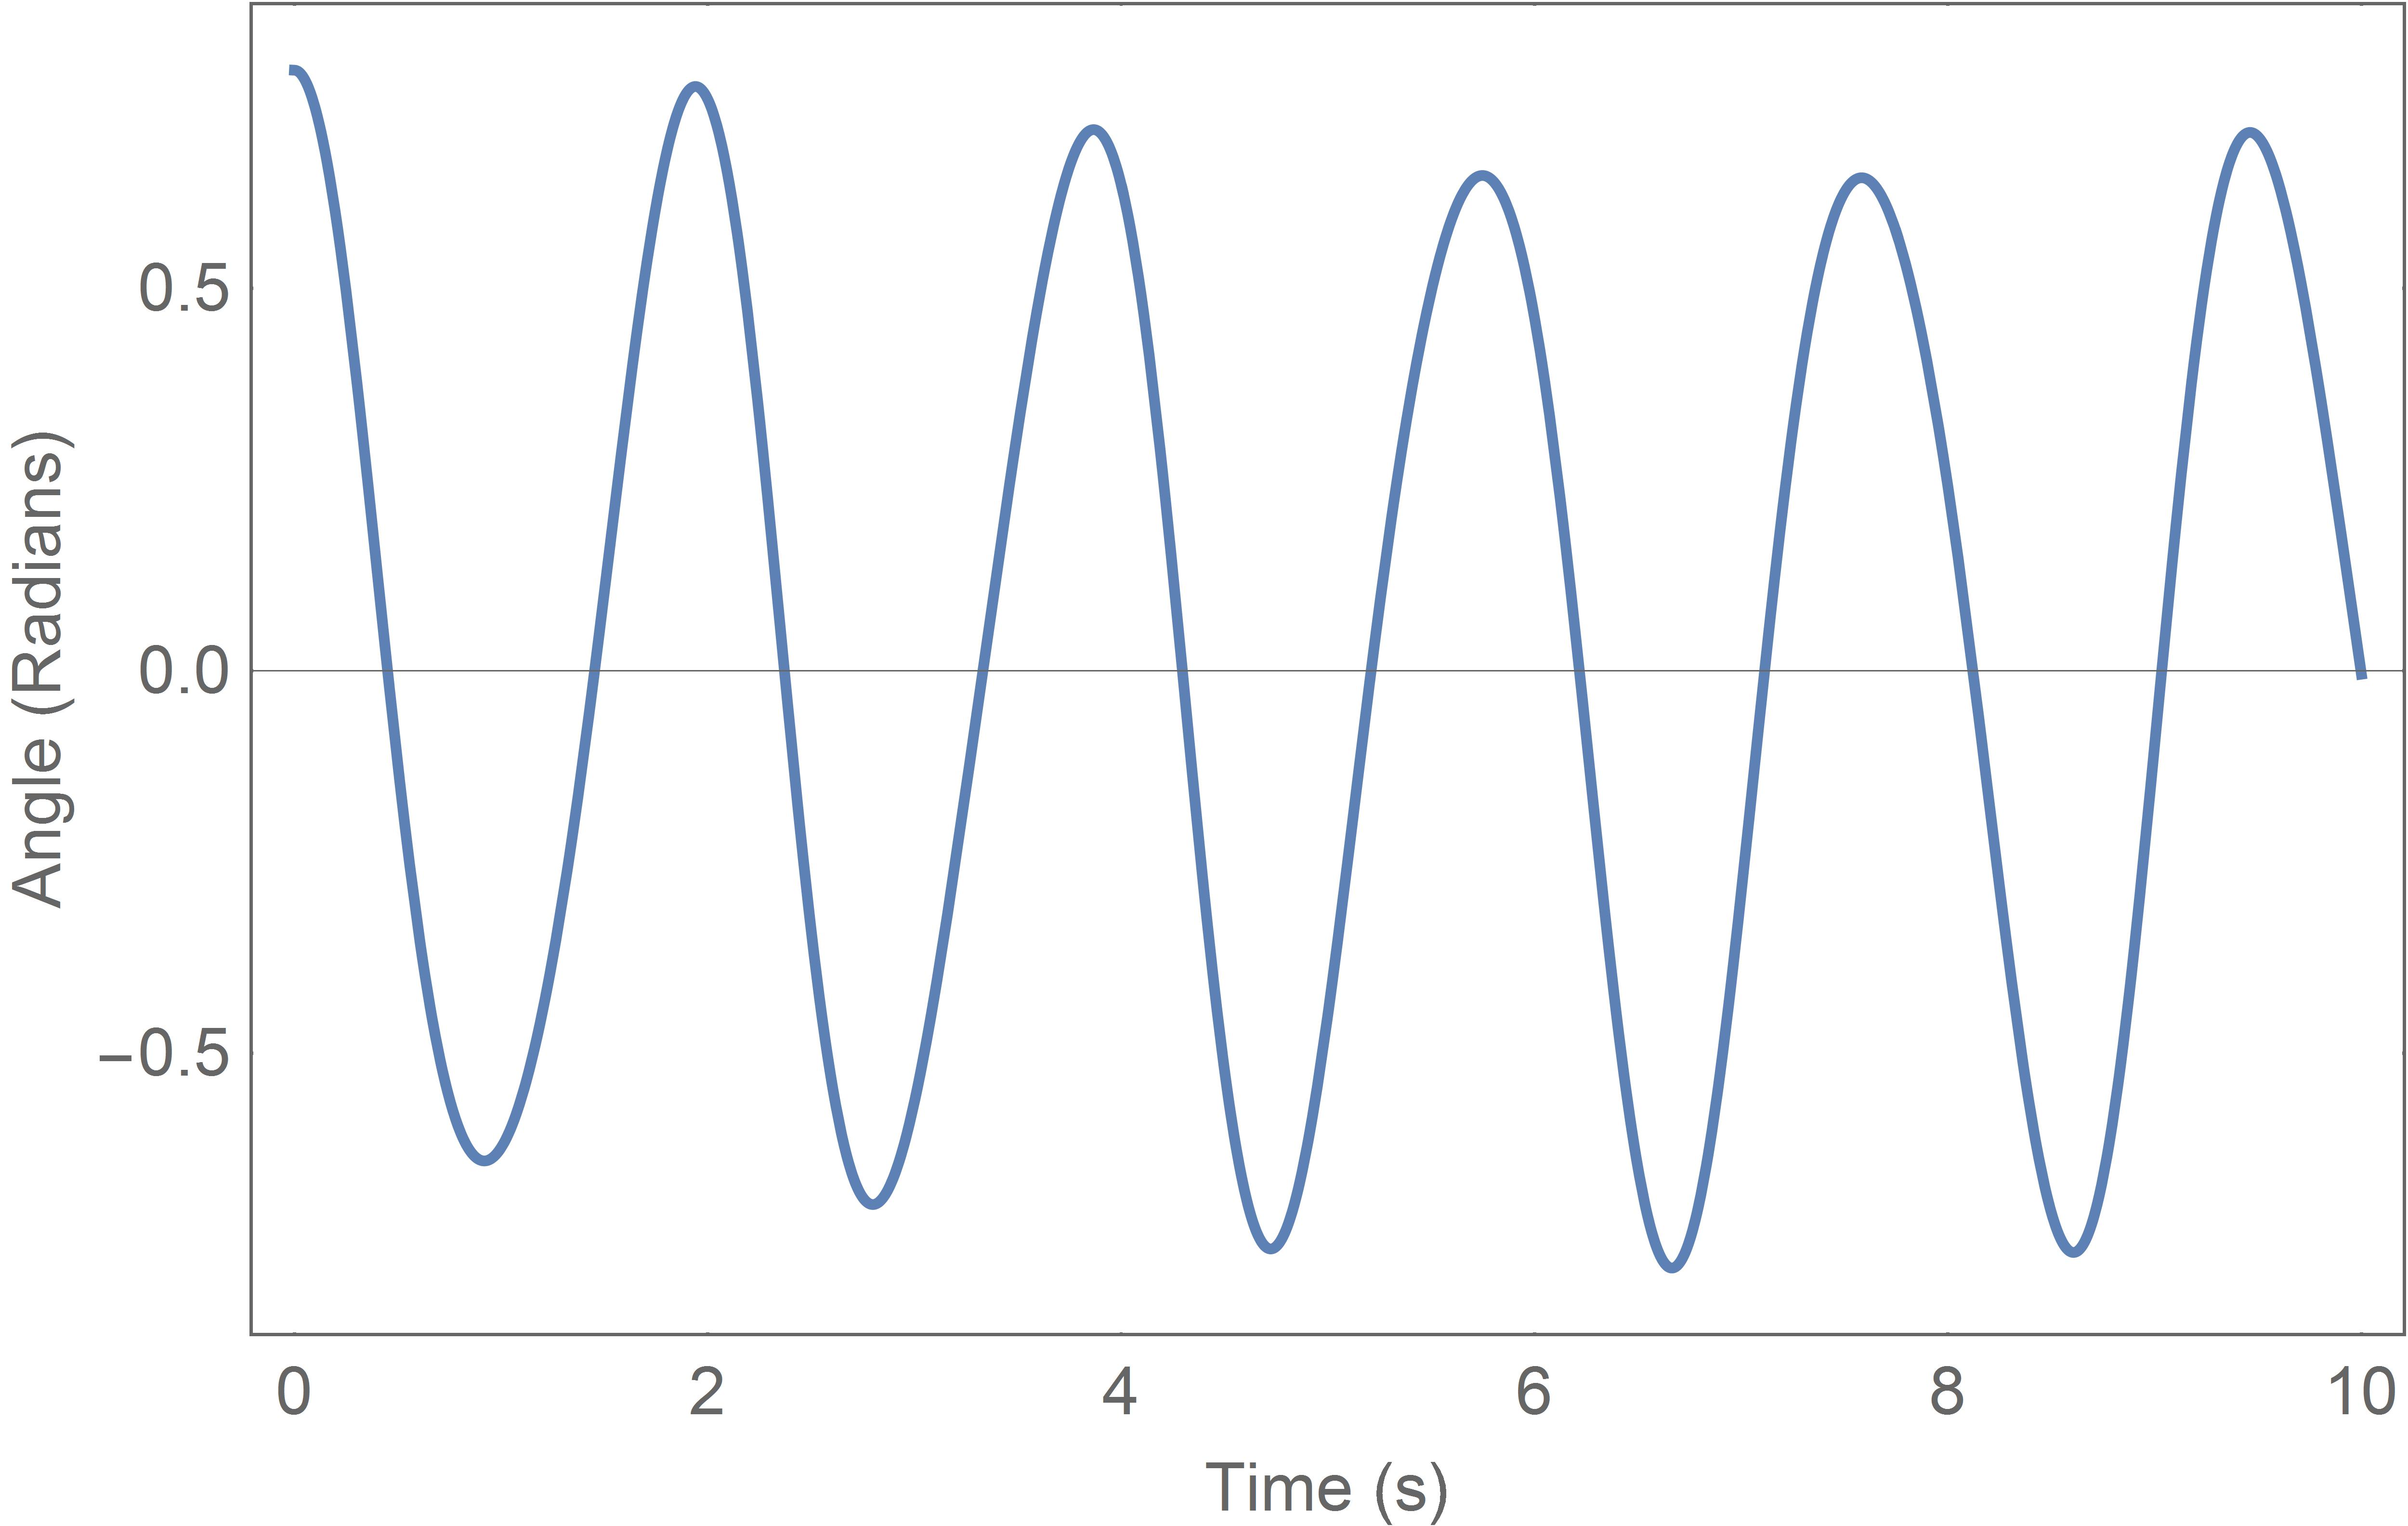
\includegraphics[width=\linewidth]{alphafp}
	\endminipage\hspace{1em}%
	\minipage{0.4\textwidth}
	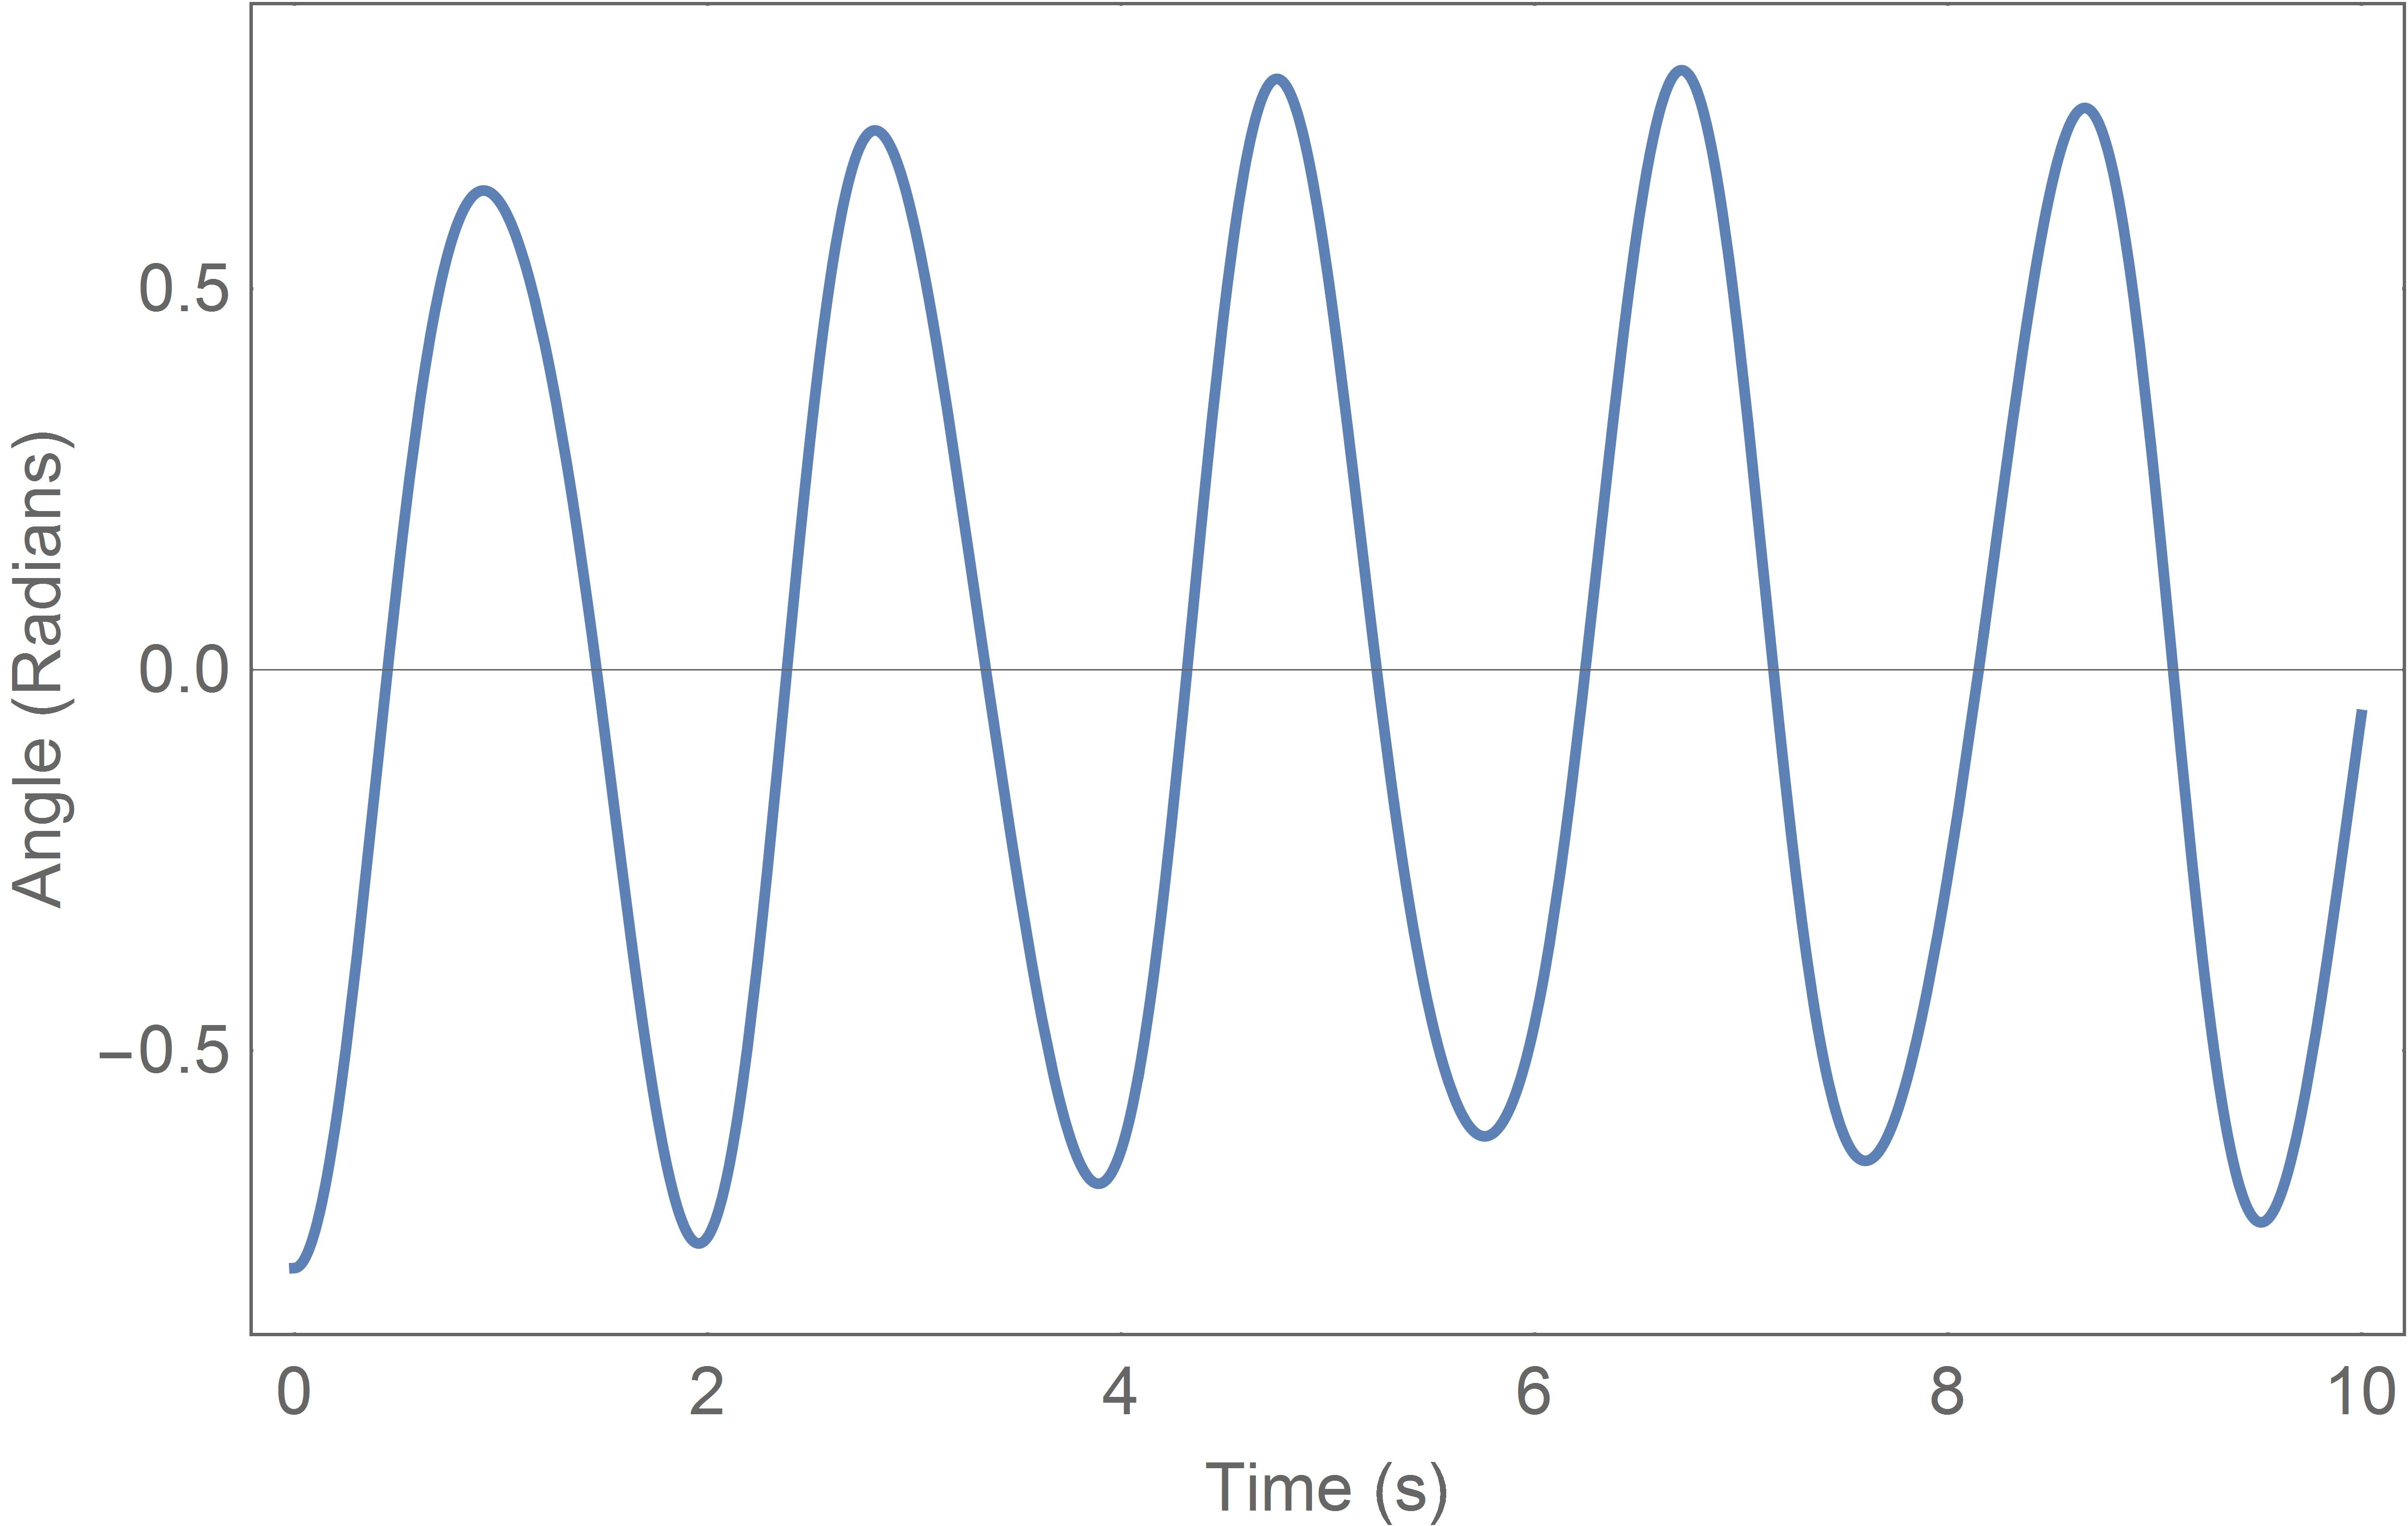
\includegraphics[width=\linewidth]{alphabp}
	\endminipage
	\caption{Roll of front plate ($\alpha_{fp}$) and back plate ($\alpha_{bp}$)}
	\label{fig:plates}
\end{figure}

\begin{figure}[!htb]
	\centering
	\minipage{0.4\textwidth}
	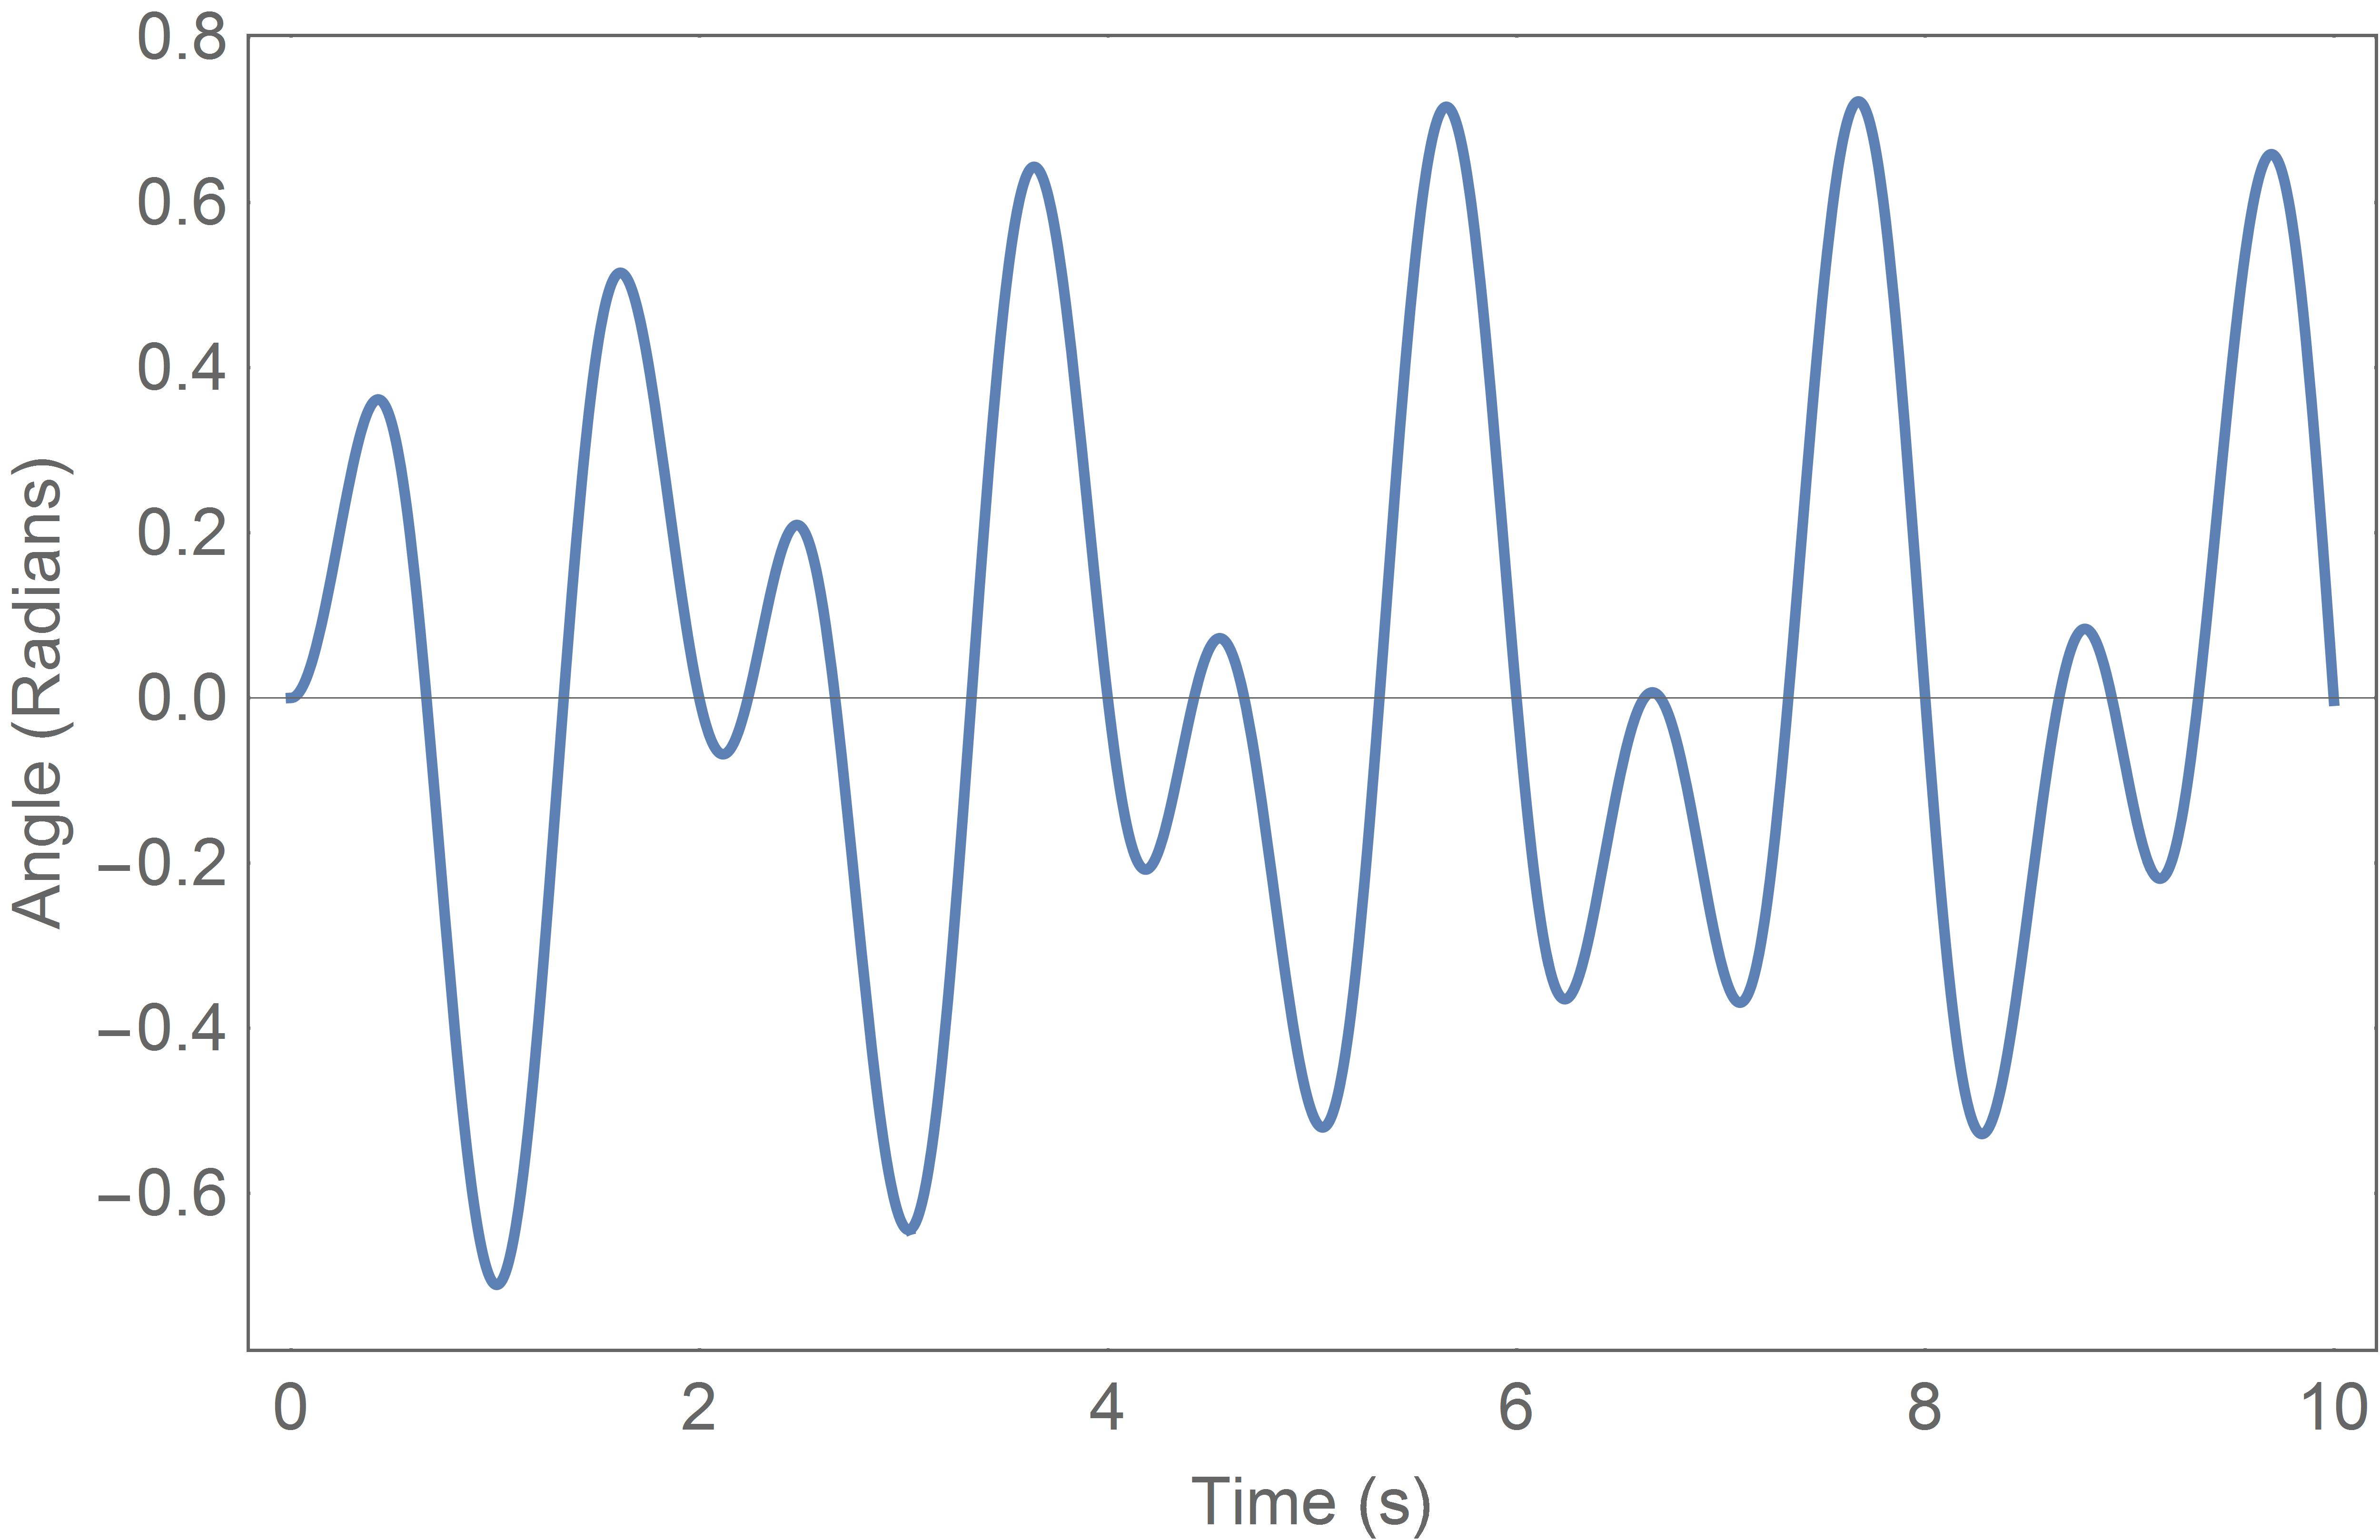
\includegraphics[width=\linewidth]{thetafc}
	\endminipage\hspace{1em}%
	\minipage{0.4\textwidth}
	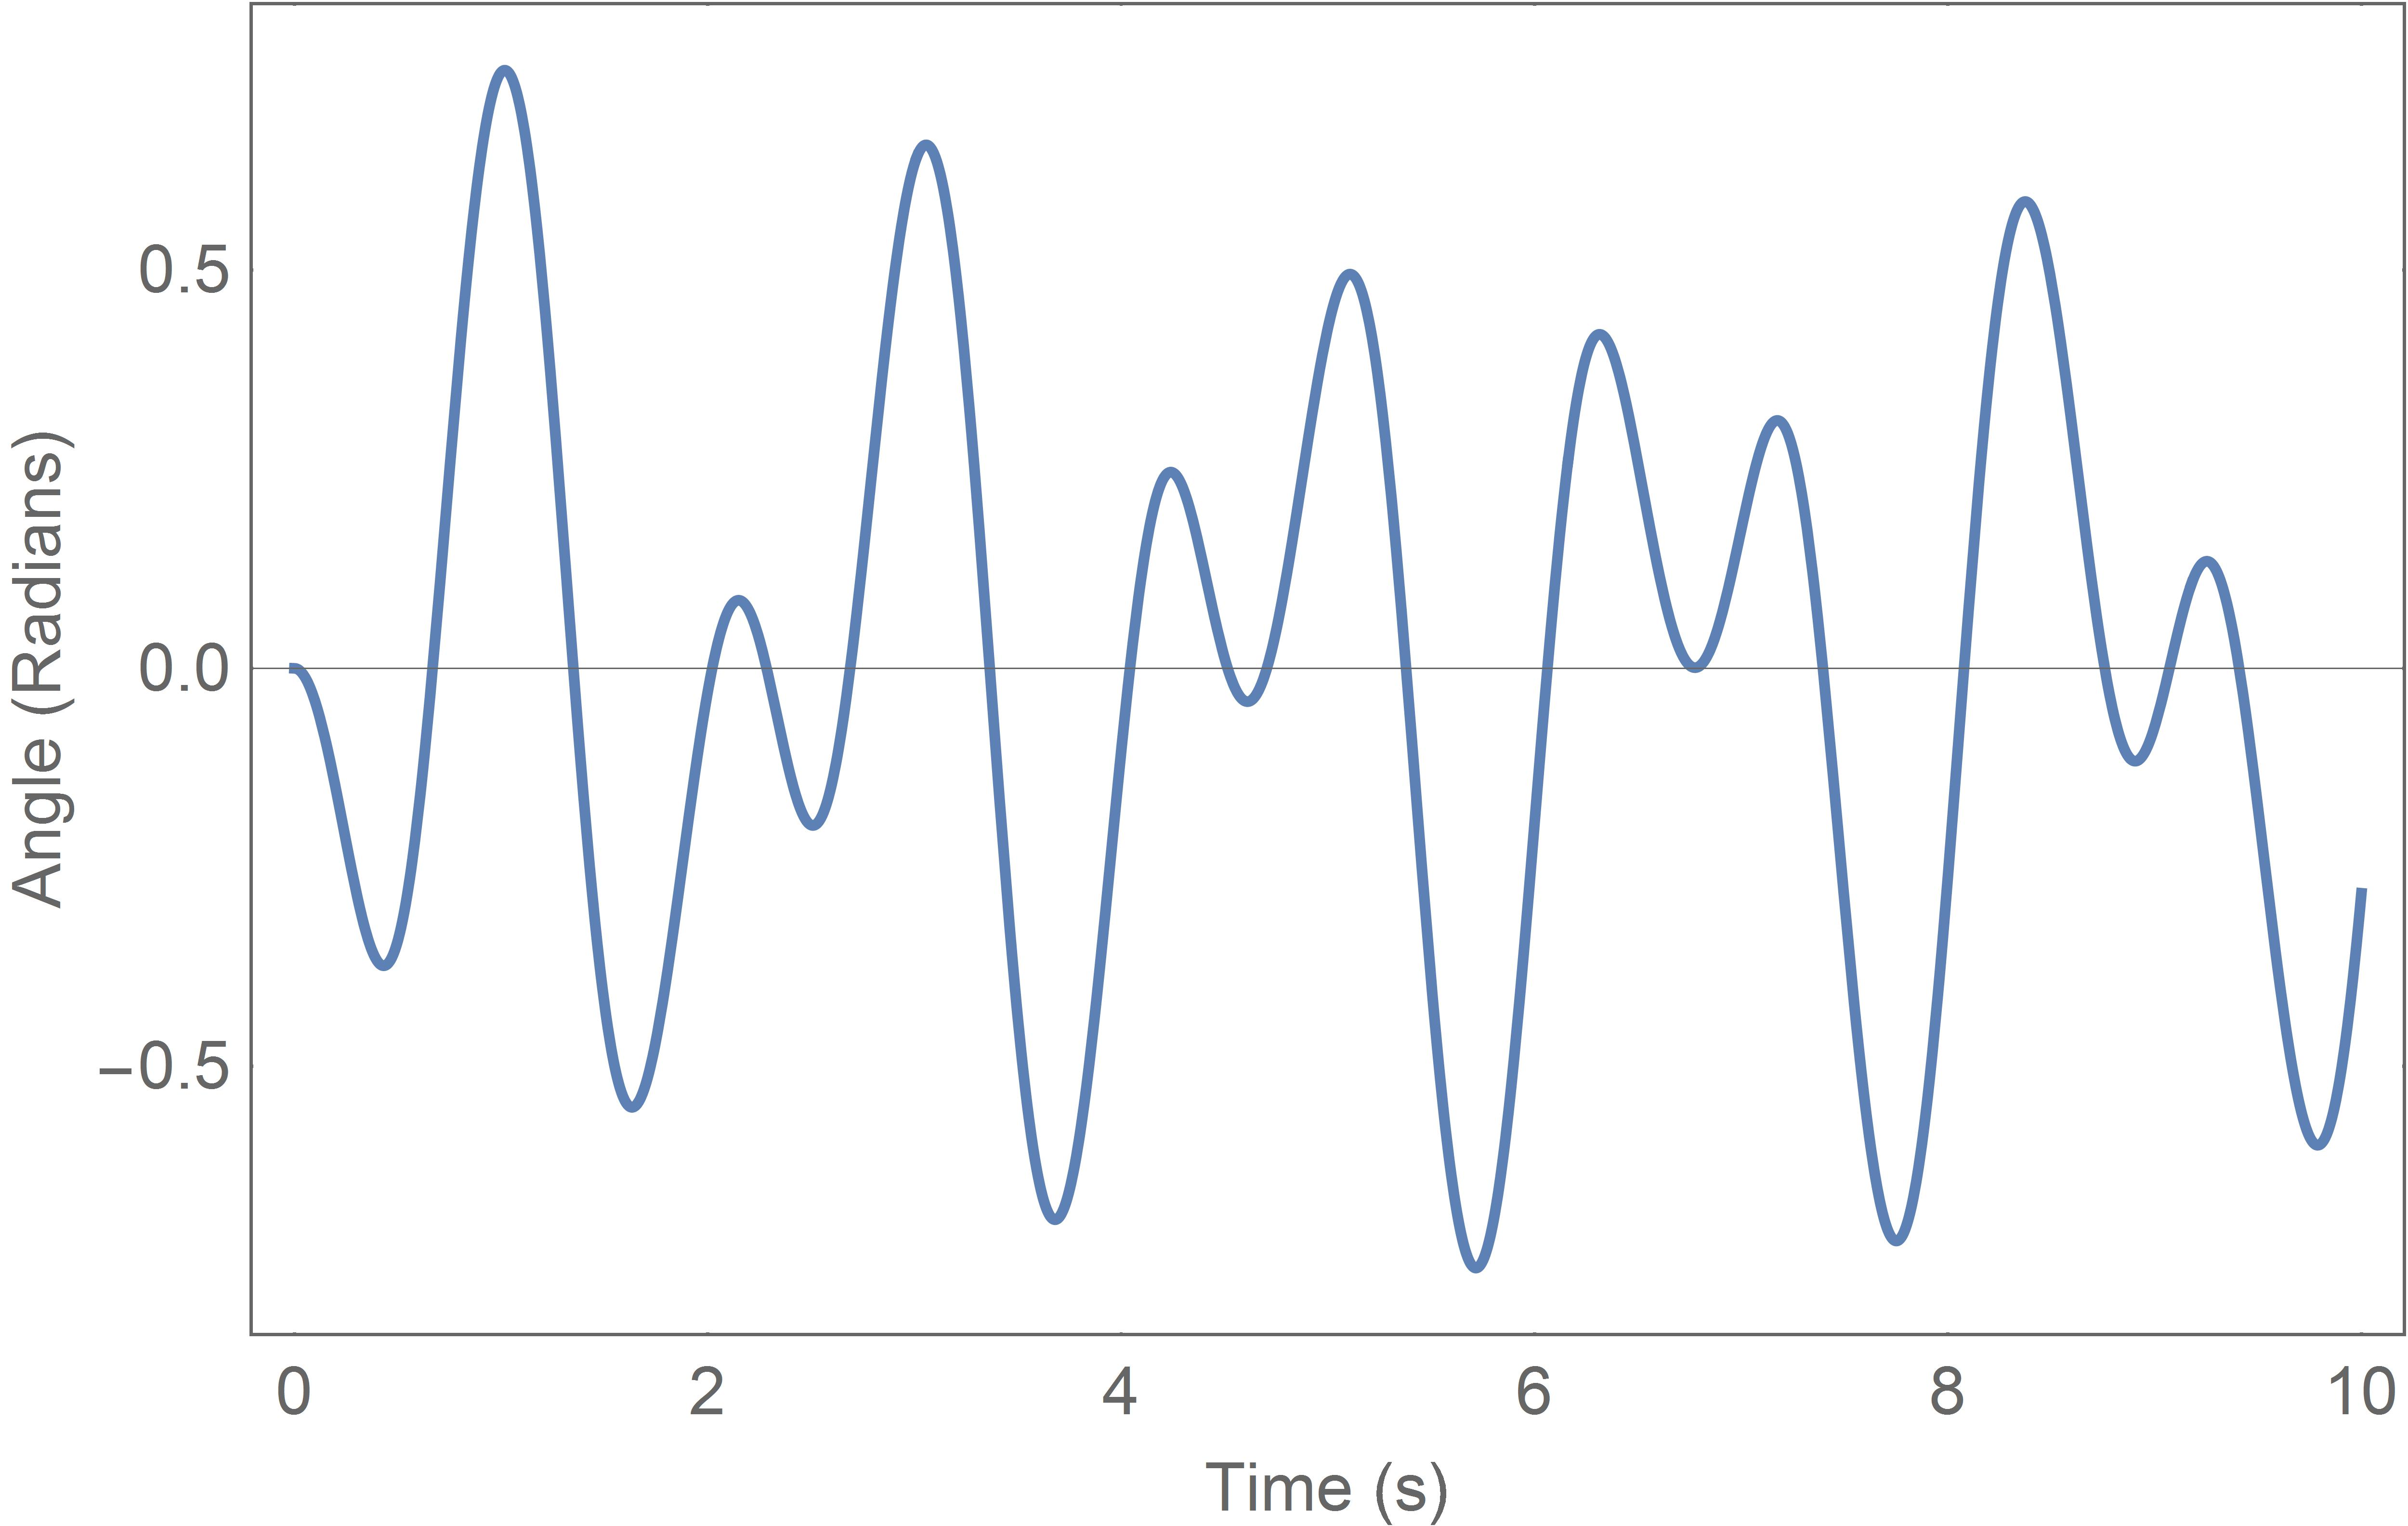
\includegraphics[width=\linewidth]{thetabc}
	\endminipage
	\caption{Yaw of front caster ($\theta_{fc}$) and back caster ($\theta_{bc}$)}
	\label{fig:casters}
\end{figure}

Since the plates and casters both experience oscillations approximately between  $\frac{\pi}{4}$ and $-\frac{\pi}{4}$, it is confirmed that the equations of motion for the RipStik are accurate.

An accurate visualization of the Ripstik is produced to model the motion. 
The two extreme positions of the RipStik is shown in Figure \ref{fig:RipStikModel1}.

\begin{figure}[!htb]
	\centering
	\minipage{0.4\textwidth}
	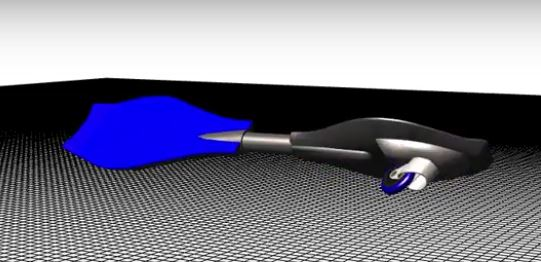
\includegraphics[width=\linewidth]{oneswing}
	\endminipage\hspace{1em}%
	\minipage{0.42\textwidth}
	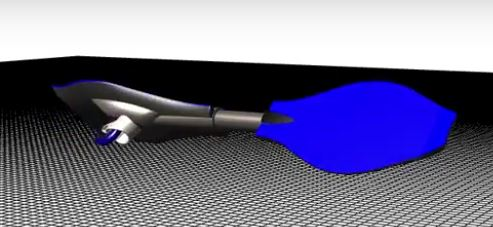
\includegraphics[width=\linewidth]{twoswing}
	\endminipage
	\caption{Two extreme positions of the RipStik motion}
	\label{fig:RipStikModel1}
\end{figure}

\subsection{Nonholonomic Constraints}

With the unconstrained equations of motion validated, nonholonomic constraints are then implemented into the system. 
The constraints are defined such that the wheels cannot slide laterally or lift off the ground. 
This represents a total of four constraint forces which are implemented using Lagrange multipliers.
Three different methods are explored when trying to solve for the nonholonomic constraints: symbolically inverting the matrices, representing the constraints as a system of linear equations $(Ax=B)$, and numeric integration.

\paragraph{Symbolic Matrix Inversion}\mbox{}\\
The initial method explored involves symbolically inverting matrices in Mathematica. First, the acceleration terms in the equations of motion are isolated. 
They are then substituted into the derivatives of the nonholonomic constraint equations, shown in Equation \ref{eq:SMI}.

\begin{equation}
\label{eq:SMI}
\Omega \ddot{q} = -\Omega G_{jk}^{-1}\Gamma_{jkl} \dot{q}^k\dot{q}^l + \Omega G_{jk}^{-1} \Omega ^T \lambda
\end{equation}

This is an intuitive approach from a linear algebra perspective; however, it is computationally demanding for large scale systems. 
When trying to solve for the acceleration terms, the computer's RAM can fill and cause Mathematica to abandon the calculation.

%%%%%%%%%%%%%%%%%%%%%%%%%%%%%%%%%%%%%%%%%%%%%%%%%%%
%%%%%%
%%%%%% MORE SPECIFIC ABOUT WHY RAM FILLS IE DETERMINANTS. Double check equation, the coeffs look a little fucky?
%%%%%%
%%%%%%%%%%%%%%%%%%%%%%%%%%%%%%%%%%%%%%%%%%%%%%%%%%%
\paragraph{System of Linear Equations $(Ax=B)$}\mbox{}\\
The next method requires taking the matrix inversion and representing it as a system of linear equations of the form $Ax=b$.
In this equation, $A$ is a square matrix and $b$ is a column vector.
This allows Mathematics more flexibility to internally choose from three different approaches for isolating the desired results: using Laplace cofactor expansion, Bareiss method of division-free row reduction, and standard row reduction for computing determinants \cite{linearsolve}.
The Bareiss method of division-free row reduction allows for the computation of determinants without introducing fractions \cite{bareiss}.
\par
At this point, all symbolic constants in the RipStik model were replaced with measured values to further simplify computations.
Using this method, the accelerations were solved in the equations of motion, but trying to find the Lagrange multipliers in the second system exceeded computation times.

\paragraph{Numeric Integration}\mbox{}\\
The final method involves solving the system numerically.
Using this method, Equations \ref{eq:CFE} and \ref{eq:CV} can remain in their initial form.
Numeric integration functions can then be applied to approximate the result of the system of differential equations and ultimately produce output from the model.
A drawback associated with this method is that it can be a difficult process requiring careful tuning of numerical integrators and ultimately does not give explicit equations for the constraints.

\subsubsection{Test Case - Rolling Wheel}\label{sec:testcaserw}

Prior to implementing the three methods in the RipStik system, a simple model of a rolling wheel was used to validate the different approaches. For nonholonomic constraints, a code was developed and tested on the simple example of a wheel that rolls without slipping.
No slip constraints are considered to be nonholonomic, and the output can be easily compared to published results.
The configuration space for the rolling wheel consists of [$x(t)$, $y(t)$, $\theta(t)$, $\phi(t)$]. 
The system and dimensions can be seen in Figure \ref{fig:rollwheel}.

\begin{figure}[!htb]
	\centering
	\minipage{0.6\textwidth}
	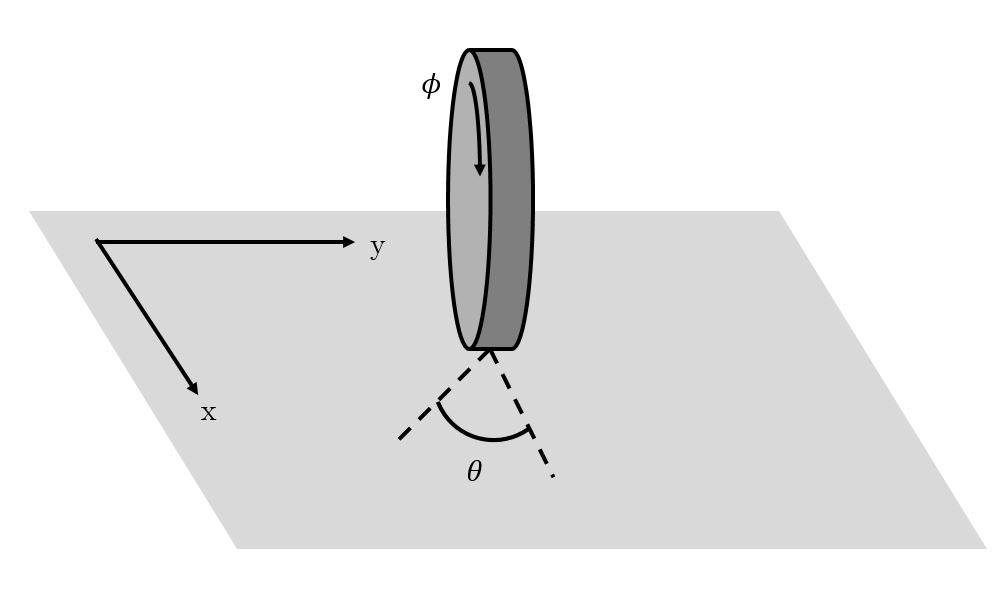
\includegraphics[width=\linewidth]{rollingwheel.JPG}
	\caption{The roll angle ($\phi$) and wheel angle ($\theta$) for the rolling wheel}\label{fig:rollwheel}
	\endminipage
\end{figure}

The Lagrangian for the system is seen in Equation \ref{eq:rollingdicks}.

\begin{equation}
\label{eq:rollingdicks}
L=\frac{1}{2}(mx'(t)^2+my'(t)^2+Jroll\theta'(t)^2+Jspin\phi'(t)^2)
\end{equation}

With the Lagrangian developed, the Euler-Lagrange equations can then be used to determine the equations of motion, as seen in Equations \ref{eq:Xroll}, \ref{eq:Yroll}, \ref{eq:thetaroll}, and \ref{eq:phiroll}.

\begin{equation}
\label{eq:Xroll}
-mx''(t)=0
\end{equation}

\begin{equation}
\label{eq:Yroll}
-my''(t)=0
\end{equation}

\begin{equation}
\label{eq:thetaroll}
-Jroll\theta''(t)=0
\end{equation}

\begin{equation}
\label{eq:phiroll}
-Jspin\phi''(t)=0
\end{equation}

Plots were then created to confirm that the rolling wheel's equations of motion with nonholonomic constraints behaved as expected.
The $x$ and $y$ positions of the rolling wheel were modelled on a parametric plot, while $\theta$ and $\phi$ were modelled on a standard plot.

\begin{figure}[!htb]
	\centering
	\minipage{0.2\textwidth}
	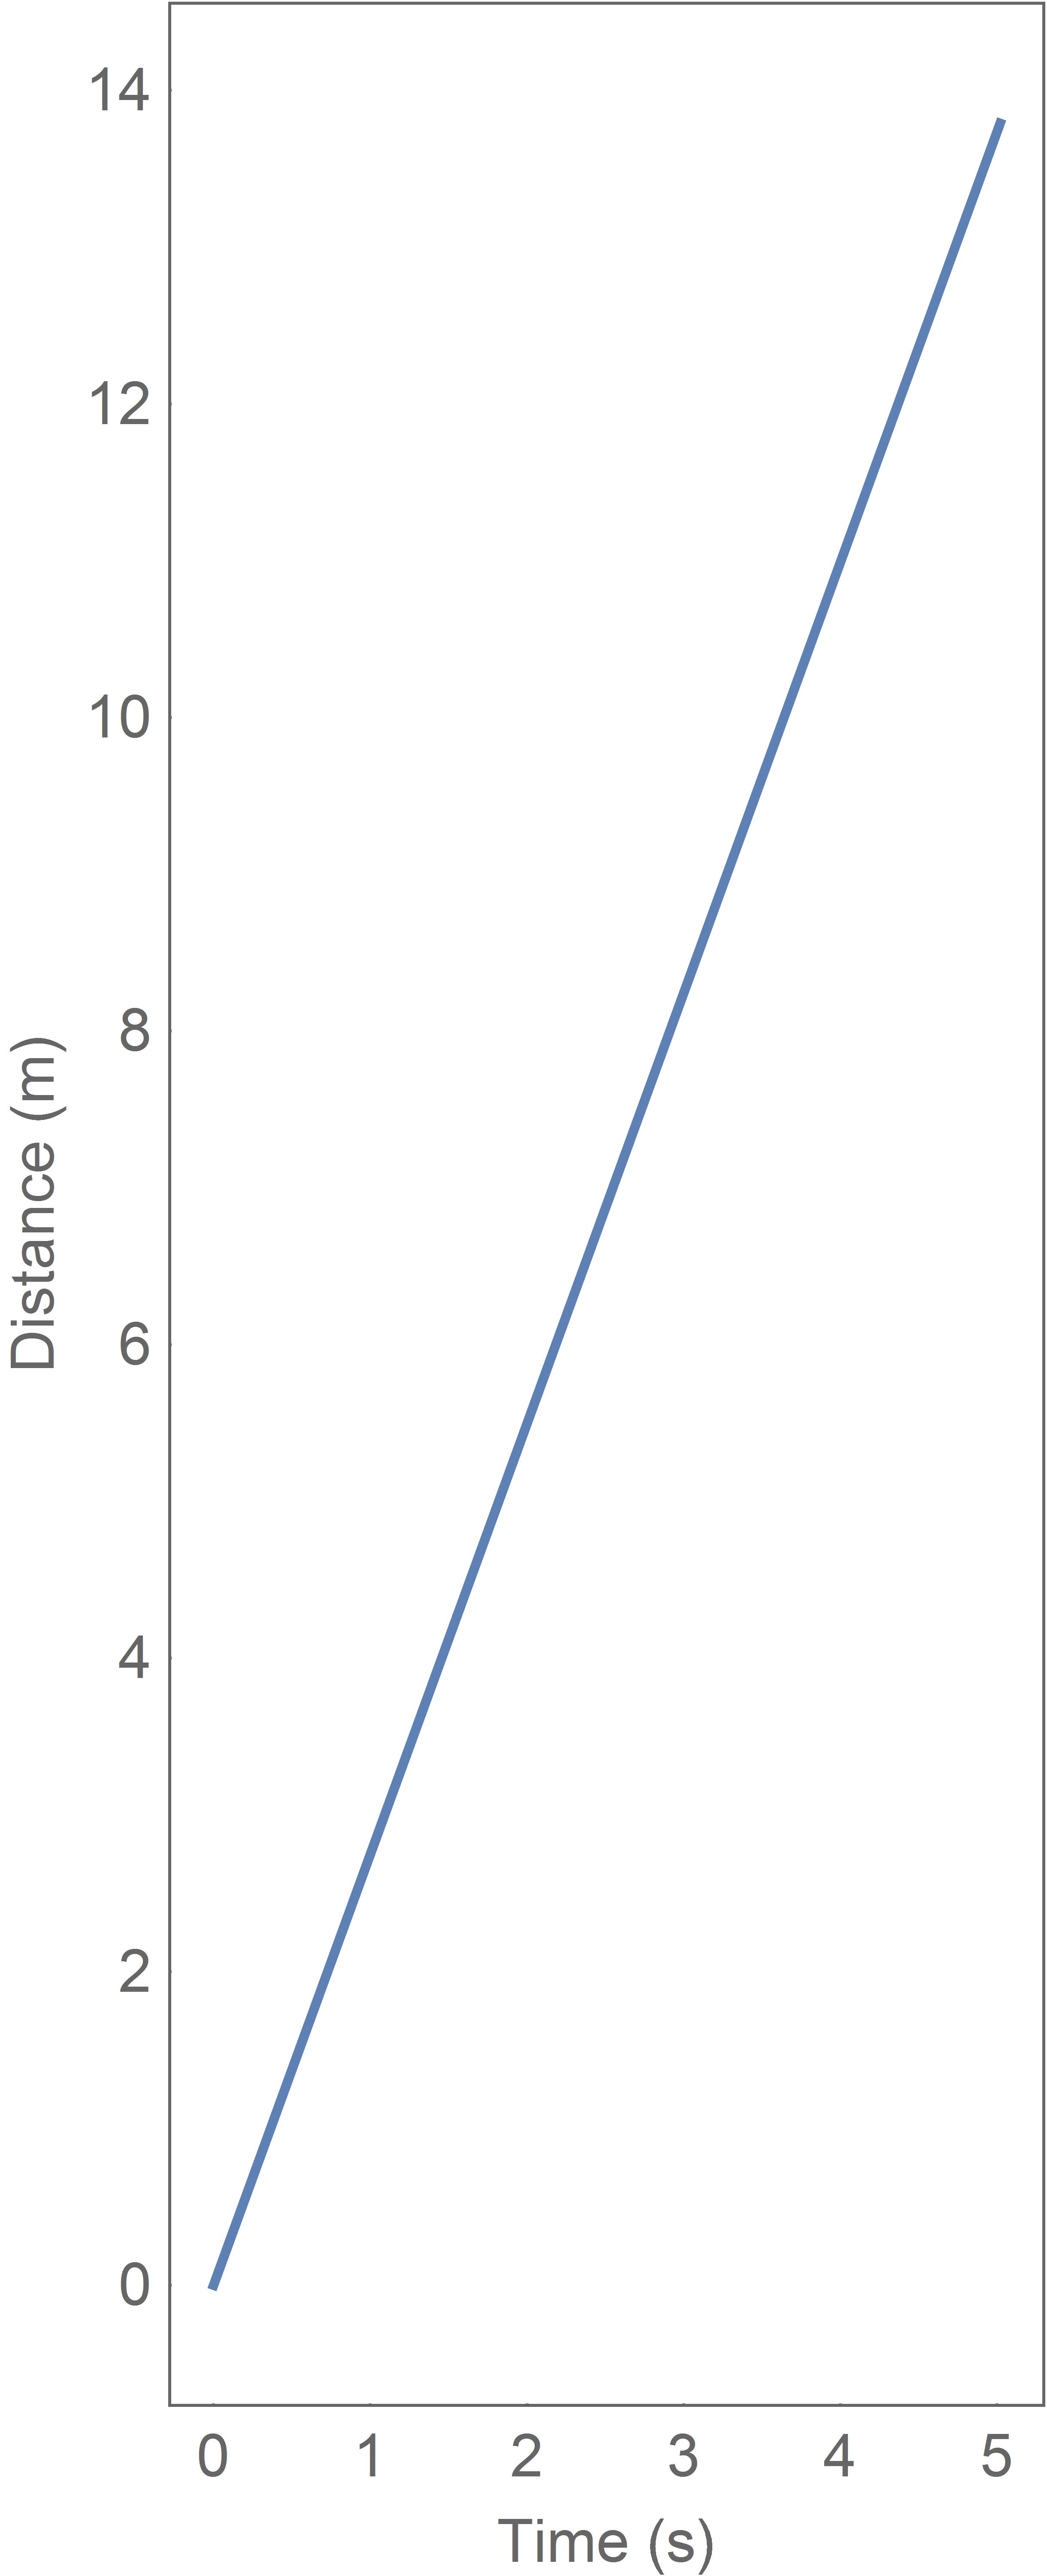
\includegraphics[width=\linewidth]{RollingWheelXY.jpg}
	\endminipage\hspace{1em}%
	\caption{The $x$ and $y$ position plotted parametrically as a function of time for 5 seconds}\label{fig:RollingWheelXY}
\end{figure}

\begin{figure}[!htb]
	\centering
	\minipage{0.4\textwidth}
	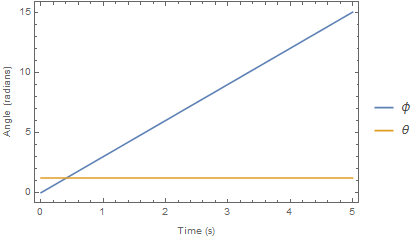
\includegraphics[width=\linewidth]{RollingWheelThetaPhi.png}
	\endminipage\hspace{1em}%
	\caption{$\theta$ and $\phi$ were plotted as a function of time for 5 seconds}\label{fig:RollingWheelThetaPhi}
\end{figure}

Based on the output in Figures \ref{fig:RollingWheelXY} and \ref{fig:RollingWheelThetaPhi}, the rolling wheel behaves as expected. 


\subsubsection{Model Implementation}

While all three approaches worked perfectly on the rolling wheel, they did not scale as desired to the much larger RipStik system.
The complexity of the system led to computations that exceeded the computer's abilities for the symbolic matrix inversion and system of linear equations.
Ultimately, numeric integration was selected to produce output.

\subsubsection{Numeric Integration}

Numeric Integration allows for the approximate computation of an integral using numerical methods \cite{WolframNumeric}.
When applying numeric integration to a differential system, stiffness is often a by-product.
The concept of stiffness is not well understood, but can generally be attributed to quick changing dynamics in a system \cite{StiffSystem}.
\par
Figure \ref{fig:stiffsystem} can be used to aid in developing an understanding of the behaviour of stiff systems. 
\begin{figure}[!htb]
	\centering
	\minipage{0.7\textwidth}
	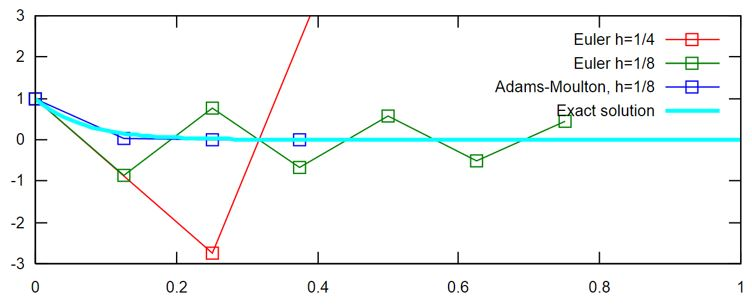
\includegraphics[width=\linewidth]{stiffsystem.JPG}
	\caption{Using numeric integration methods to approximate the exact solution to a differential equation}\label{fig:stiffsystem}
	\endminipage
\end{figure}
Figure \ref{fig:stiffsystem} shows the exact output from a simple differential equation in light blue. 
When numeric integration is attempted using Euler's method and a step size of 1/4, represented by the red line, the approximation oscillates and overshoots the exact method.
When a step size of 1/8 is selected, represented by the green line, oscillations are still present, but they are in a reasonable range around the exact solution. 
When Adams-Moulton method is used with a step size of 1/8, the oscillations are essentially negligible and the approximation is nearly identical to the exact solution.


\par
When a system has quickly changing dynamics, numeric integration requires increasingly small step sizes to approximate a solution without instability \cite{StiffSystem}. 
This adds computational complexity that often exceeds modern technological capabilities. 
To try and reduce this computational complexity, four different numerical methods are selected to evaluate stiff differential algebraic equation (DAE) systems.

The QR Decomposition method decomposes the Jacobian of the derivative, breaking down the core system into two smaller systems at each iteration point \cite{Methods}.
This is represented by the following equation:

\begin{equation}
\label{eq:QR}
A = QR
\end{equation}

In Equation \ref{eq:QR}, $A$ is any real square matrix, $Q$ is an orthogonal matrix, and $R$ is an upper triangular matrix \cite{Methods}.

The Collocation method linearizes the implicit DAE to $m$ points in time, generating a system of linear equations which can be solved iteratively using Newton's Method \cite{Methods}.
The Implicit Differential-Algebraic Method uses Backward Differential Formulas (BDF) to implicitly solve the DAE for derivatives to use an ODE solver \cite{Methods}. 
The BDF approximates the derivative of the function using information from previous time steps \cite{Methods}.
The BLT Method puts the system into block lower triangular form and solves subsets of the system iteratively \cite{Methods}.

While numeric integration produces results for the RipStik model, it brings its own set of challenges in the form of system stiffness.
For the RipStik, the frictionless linkages cause quick changes in the exact solution that is being approximated. 
When Mathematica attempts to numerically approximate this, it selects increasingly small step sizes to replicate these quick motions without oscillation. 
However, these increasingly small step sizes slow down the computation until Mathematica eventually abandons the attempt at numerically integrating over the chosen time interval.

\paragraph{Evaluation}\mbox{}\\
As previously discussed, four methods for numerically integrating stiff DAE systems are analysed. 
QR decomposition, Collocation, IDA, and BLT methods are evaluated based on three criteria:
\begin{itemize}
\item The computation time is evaluated based on how long it takes for output to be generated (in seconds)
\item The duration of output is evaluated based on the length of the output computed (in seconds)
\item The reconfigurability of each method is evaluated qualitatively based on the number of tunable parameters that can be used to generate a greater length of output
\end{itemize}
A comparison of the results is shown in Table \ref{table:evaluation}.

\begin{table}[ht]
	\caption{Numeric Integration Method Evaluation}
	\centering
	\def\arraystretch{1.3}
	\begin{tabular}{|c| c| c| c| c|}
		\hline\hline
		& QR Decomposition & \begin{tabular}{@{}c@{}}Collocation \\ Method\end{tabular} & IDA Method & BLT Method \\ 
		\hline
		Computation Time (s) & 1.2 & 26.4 & 1.2 & 1.2\\
		\hline
		Output Duration (s) & 0.6 & 5.8 & 0.6 & 0.6\\
		\hline
		Reconfigurability & Poor & Excellent & Good & Poor\\ [0.1ex]
		\hline
	\end{tabular}
	\label{table:evaluation}
\end{table}
From the results in table \ref{table:evaluation}, it is clear that there is a definitive trade-off between computation time and length of output.
The Collocation method is able to produce an output 9.7 times longer than all other methods, at a cost of 22 times longer computation.  
The gain in length of output is weighted far greater than the length of computation time, since the lengthened computation time was still feasible.

\subsubsection{Validation}

Using the Collocation integration method, 5.8 seconds of output for the falling RipStik is generated for each degree of freedom in the system. 
As the RipStik falls however, it eventually exceeds the range of validity for the Euler angles. 
This leads to the RipStik's motion behaving erratically. 
As a result, only the first 1.4 seconds of the falling RipStik are plotted.

\begin{figure}[!htb]
	\centering
	\minipage{0.4\textwidth}
	\includegraphics[width=\linewidth]{fallz}
	\endminipage\hspace{1em}%
	\caption{The $z$-position of the Ripstik as it falls}\label{fig:fallglobal}
\end{figure}

\begin{figure}[!htb]
	\centering
	\minipage{0.4\textwidth}
	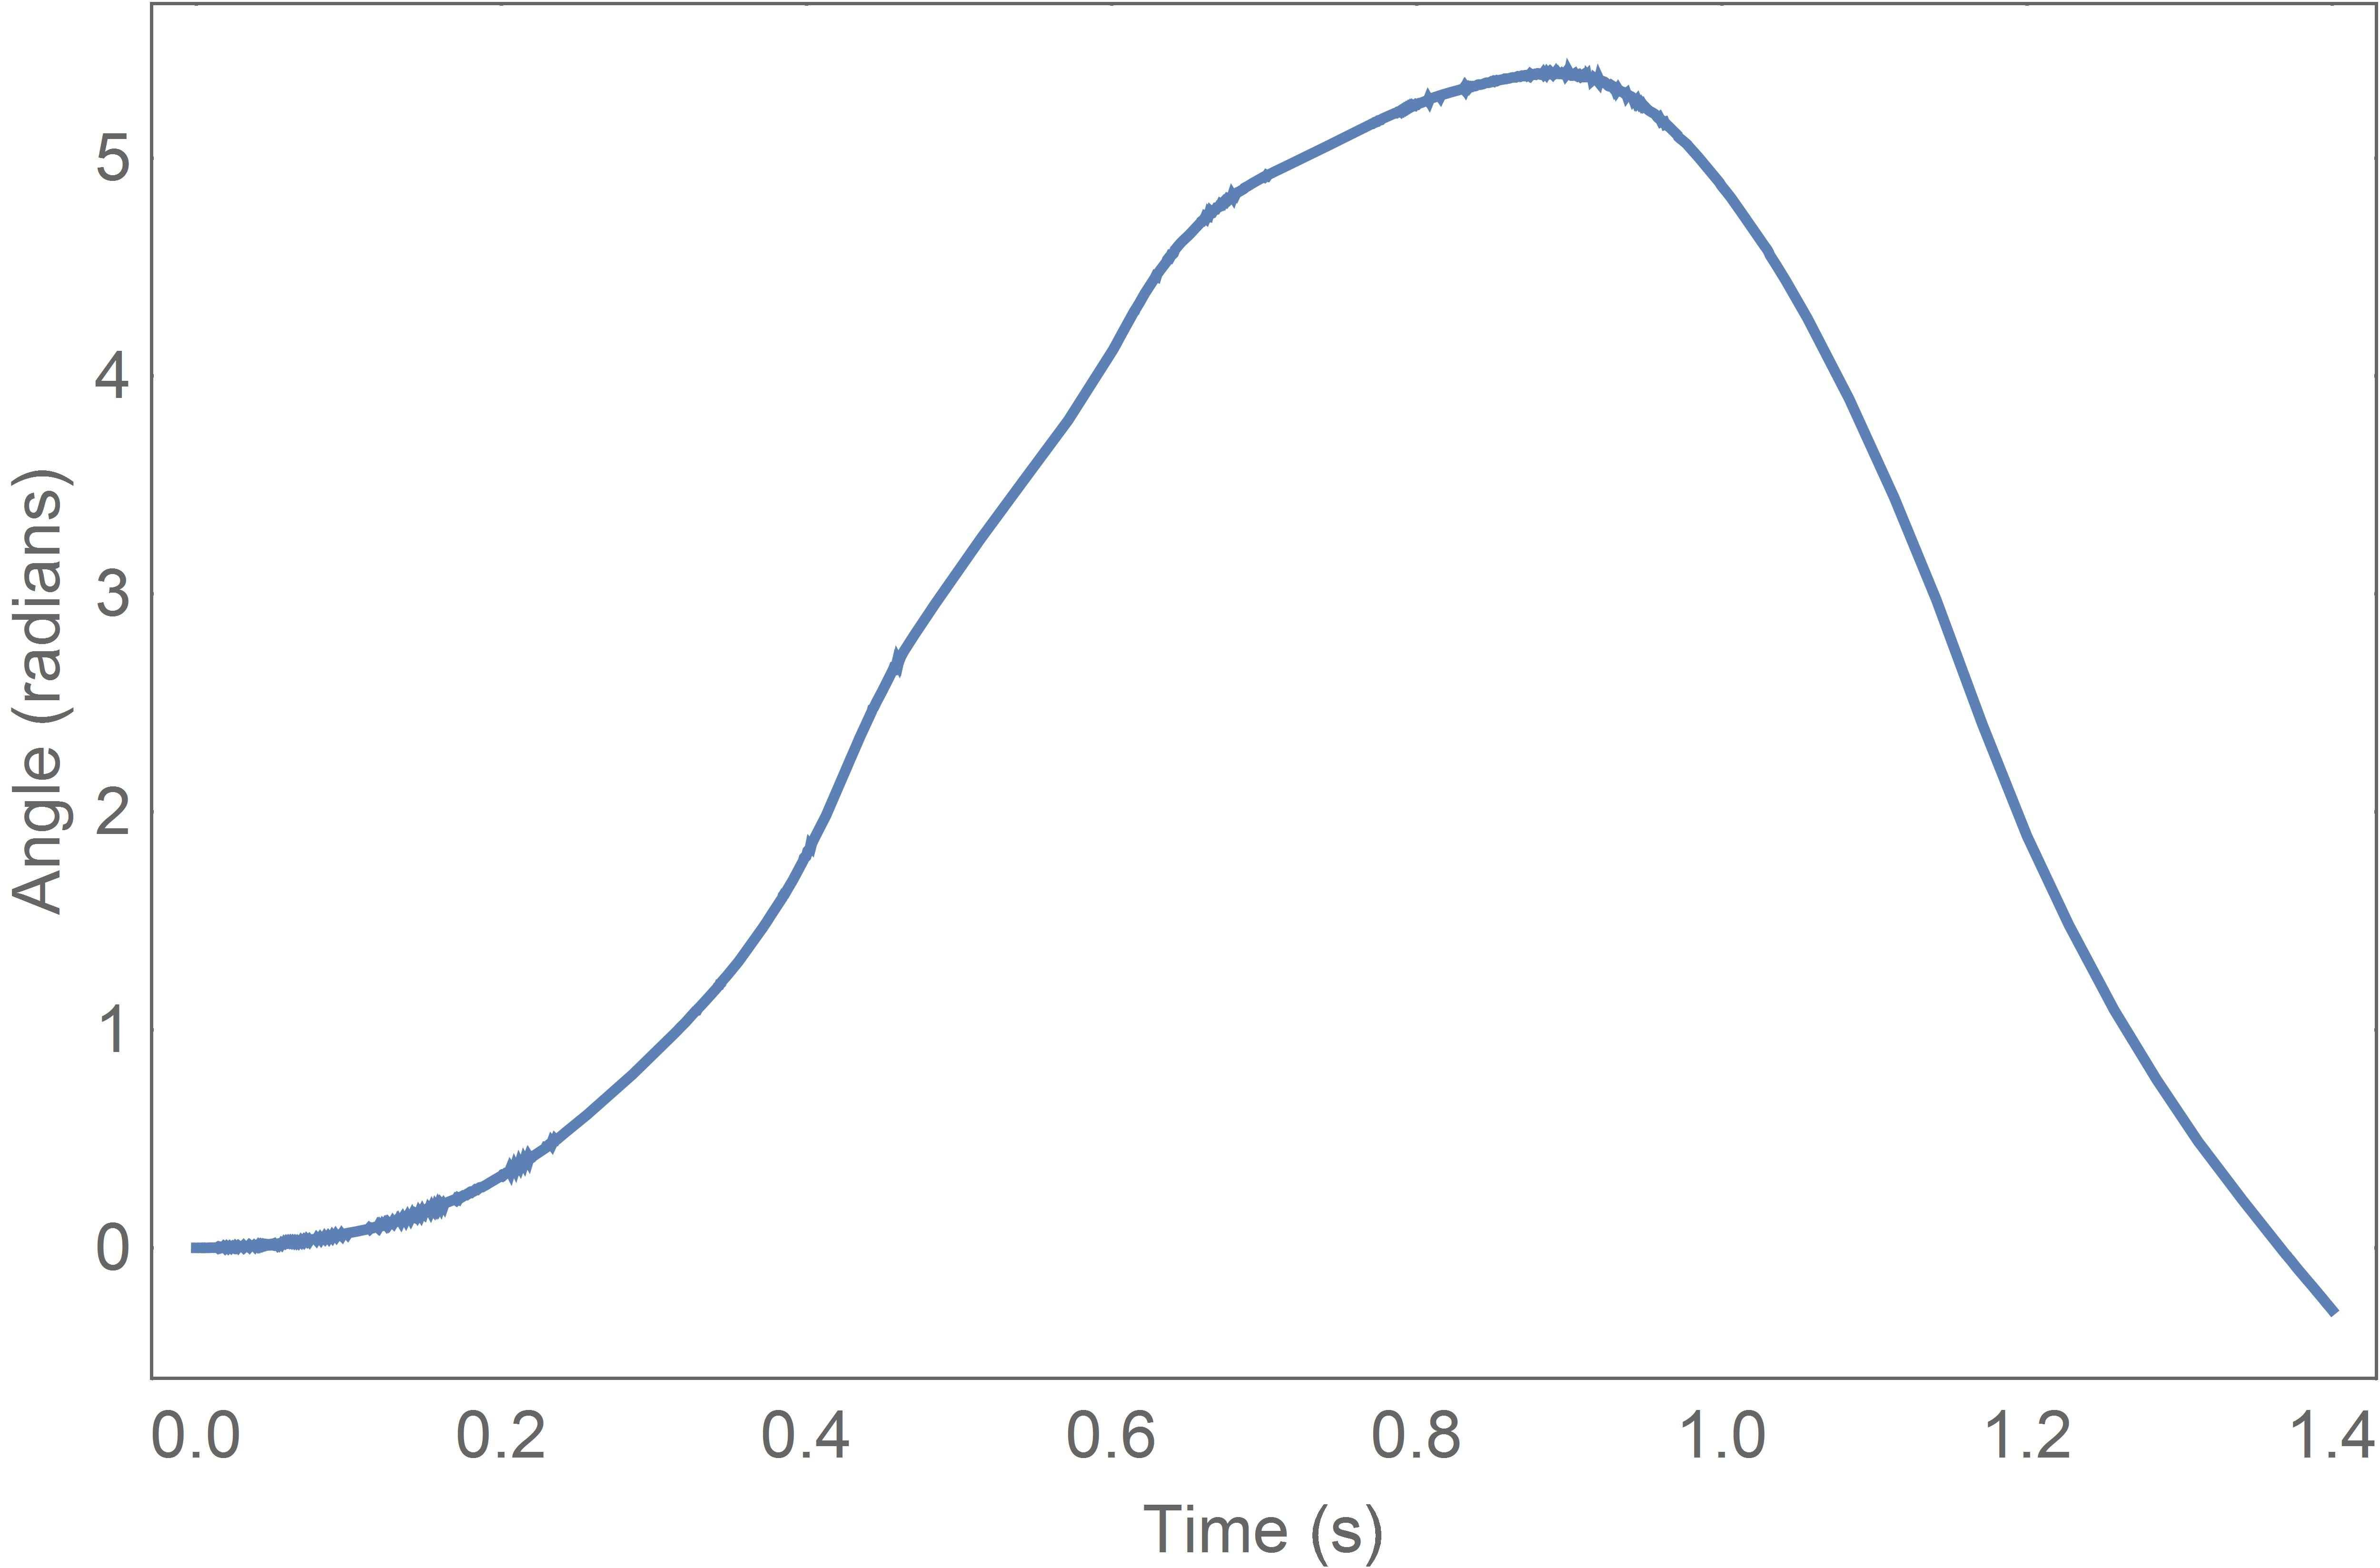
\includegraphics[width=\linewidth]{fallalphafp}
	\endminipage\hspace{1em}%
	\minipage{0.4\textwidth}
	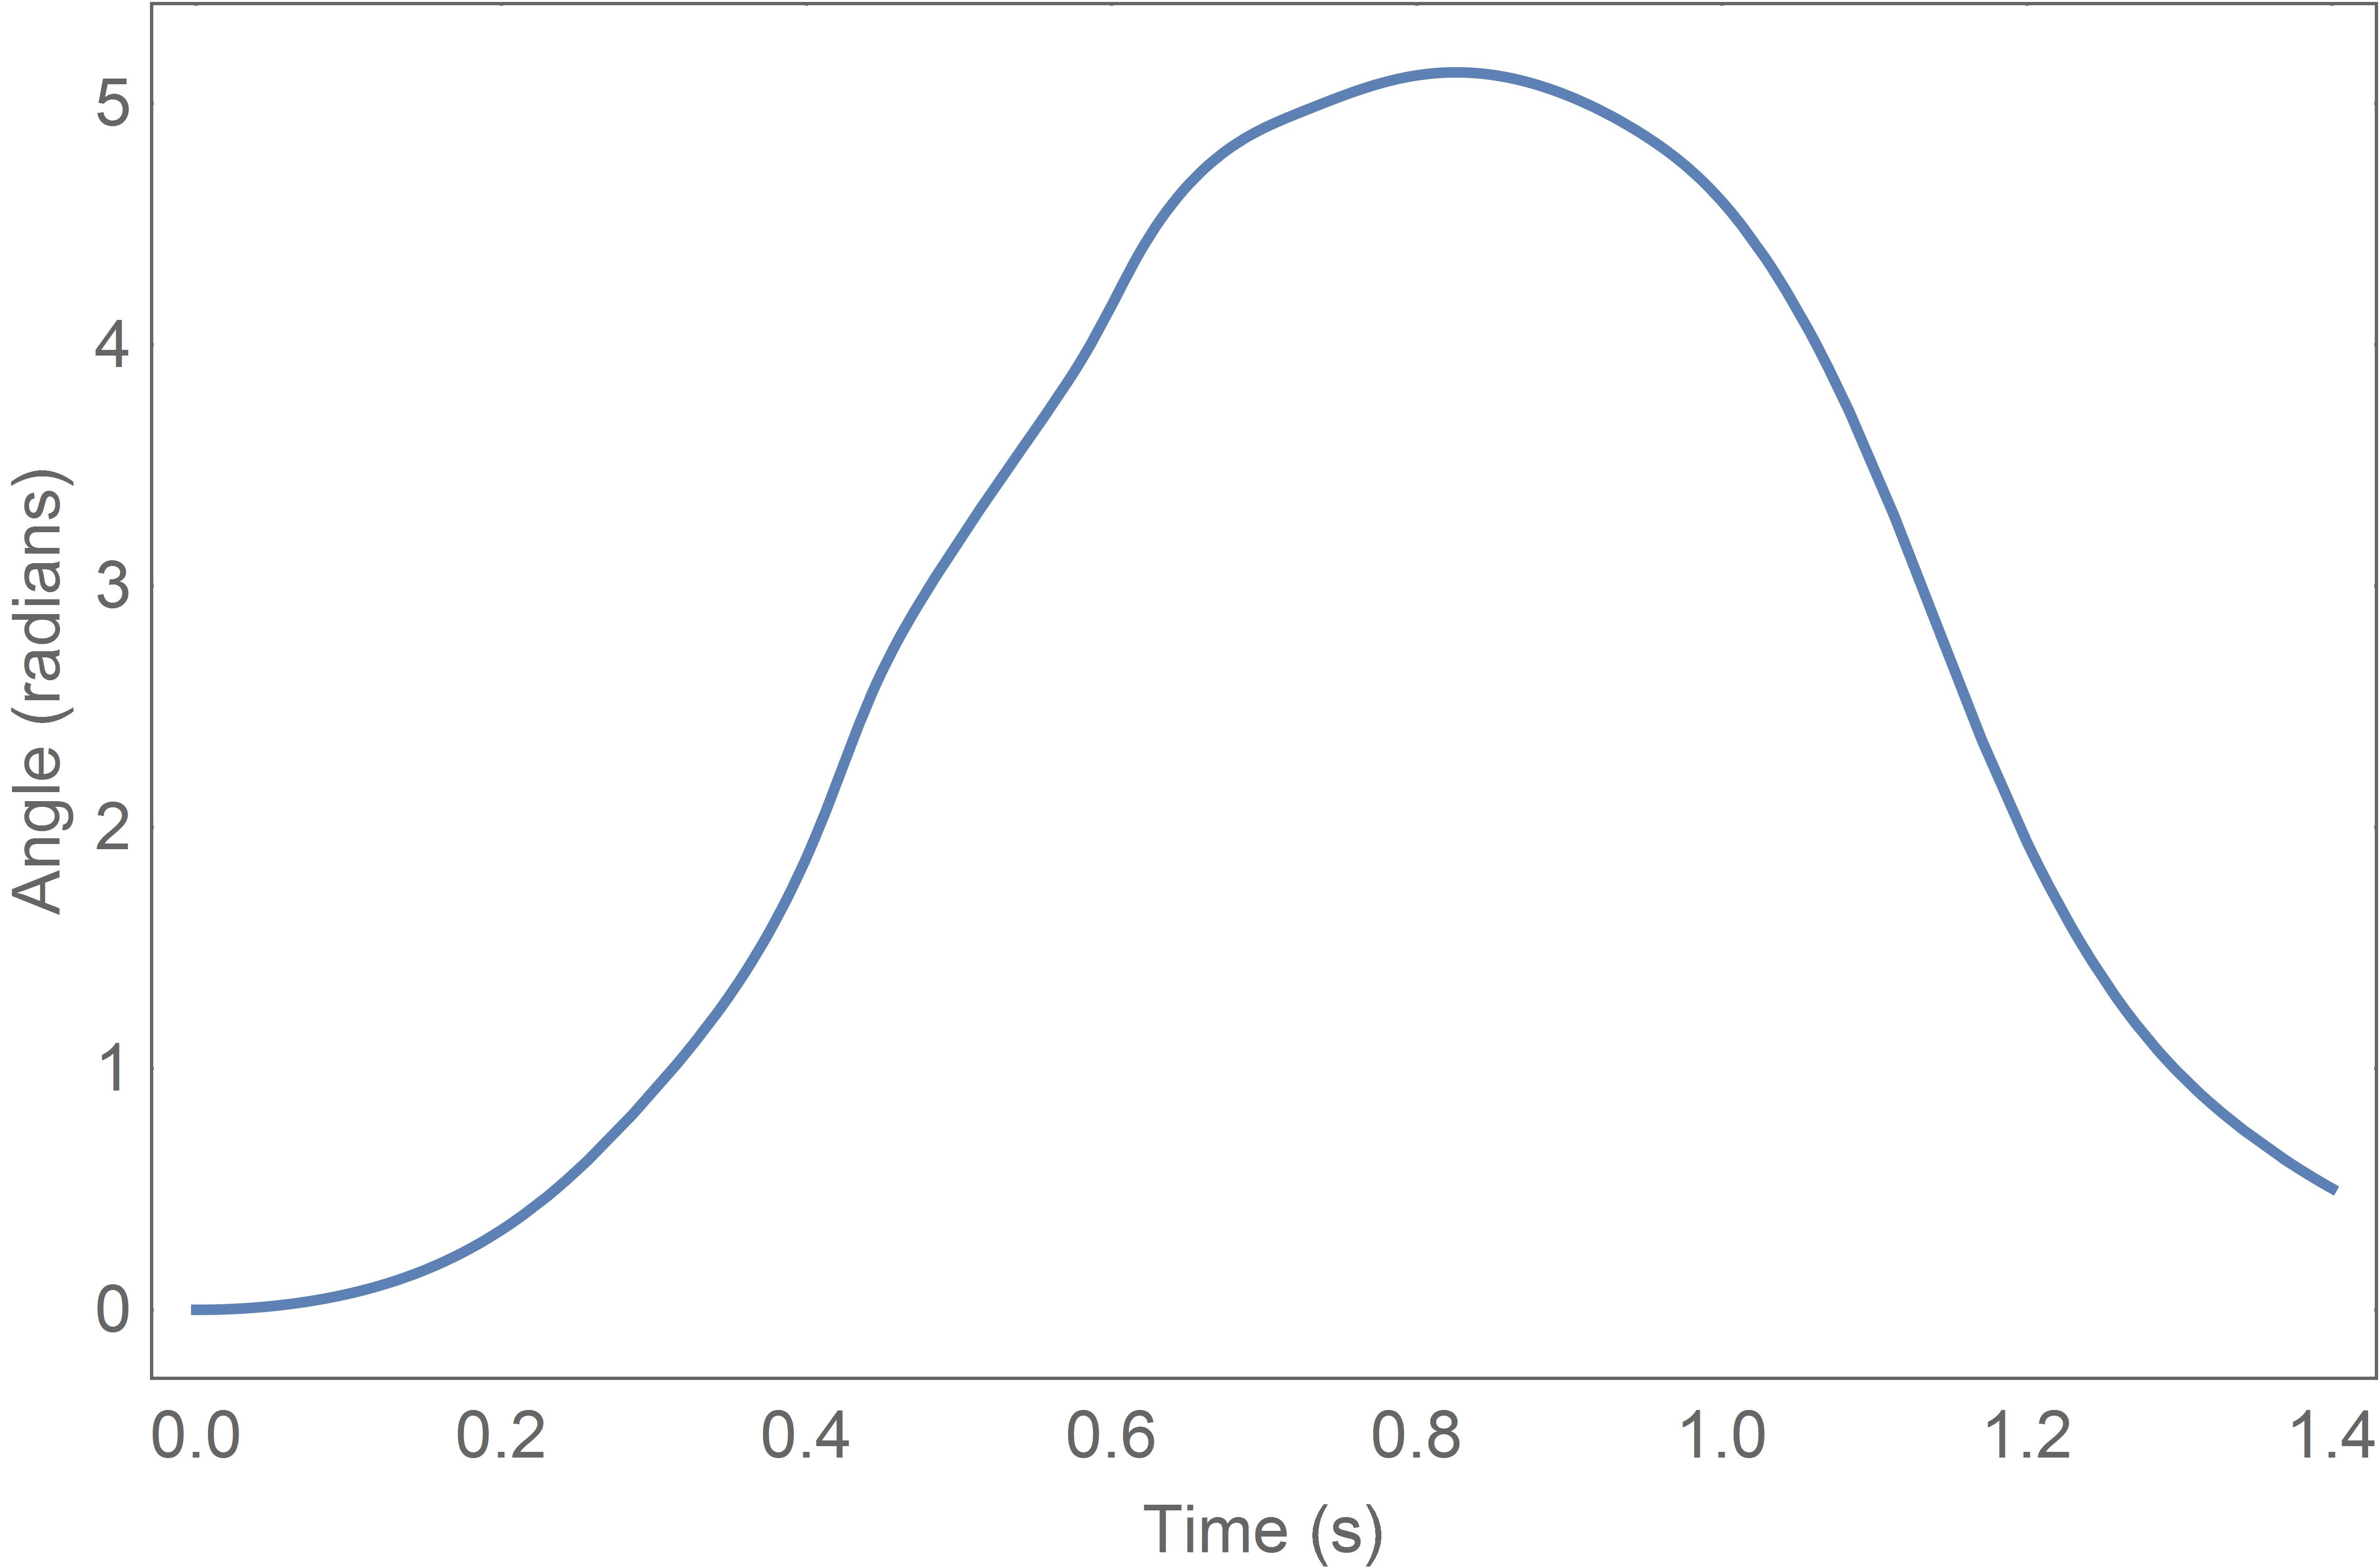
\includegraphics[width=\linewidth]{fallalphabp}
	\endminipage
	\caption{Roll of front plate ($\alpha_{fp}$) and back plate ($\alpha_{bp}$) as the RipStik falls}\label{fig:fallplates}
\end{figure}

\begin{figure}[!htb]
	\centering
	\minipage{0.4\textwidth}
	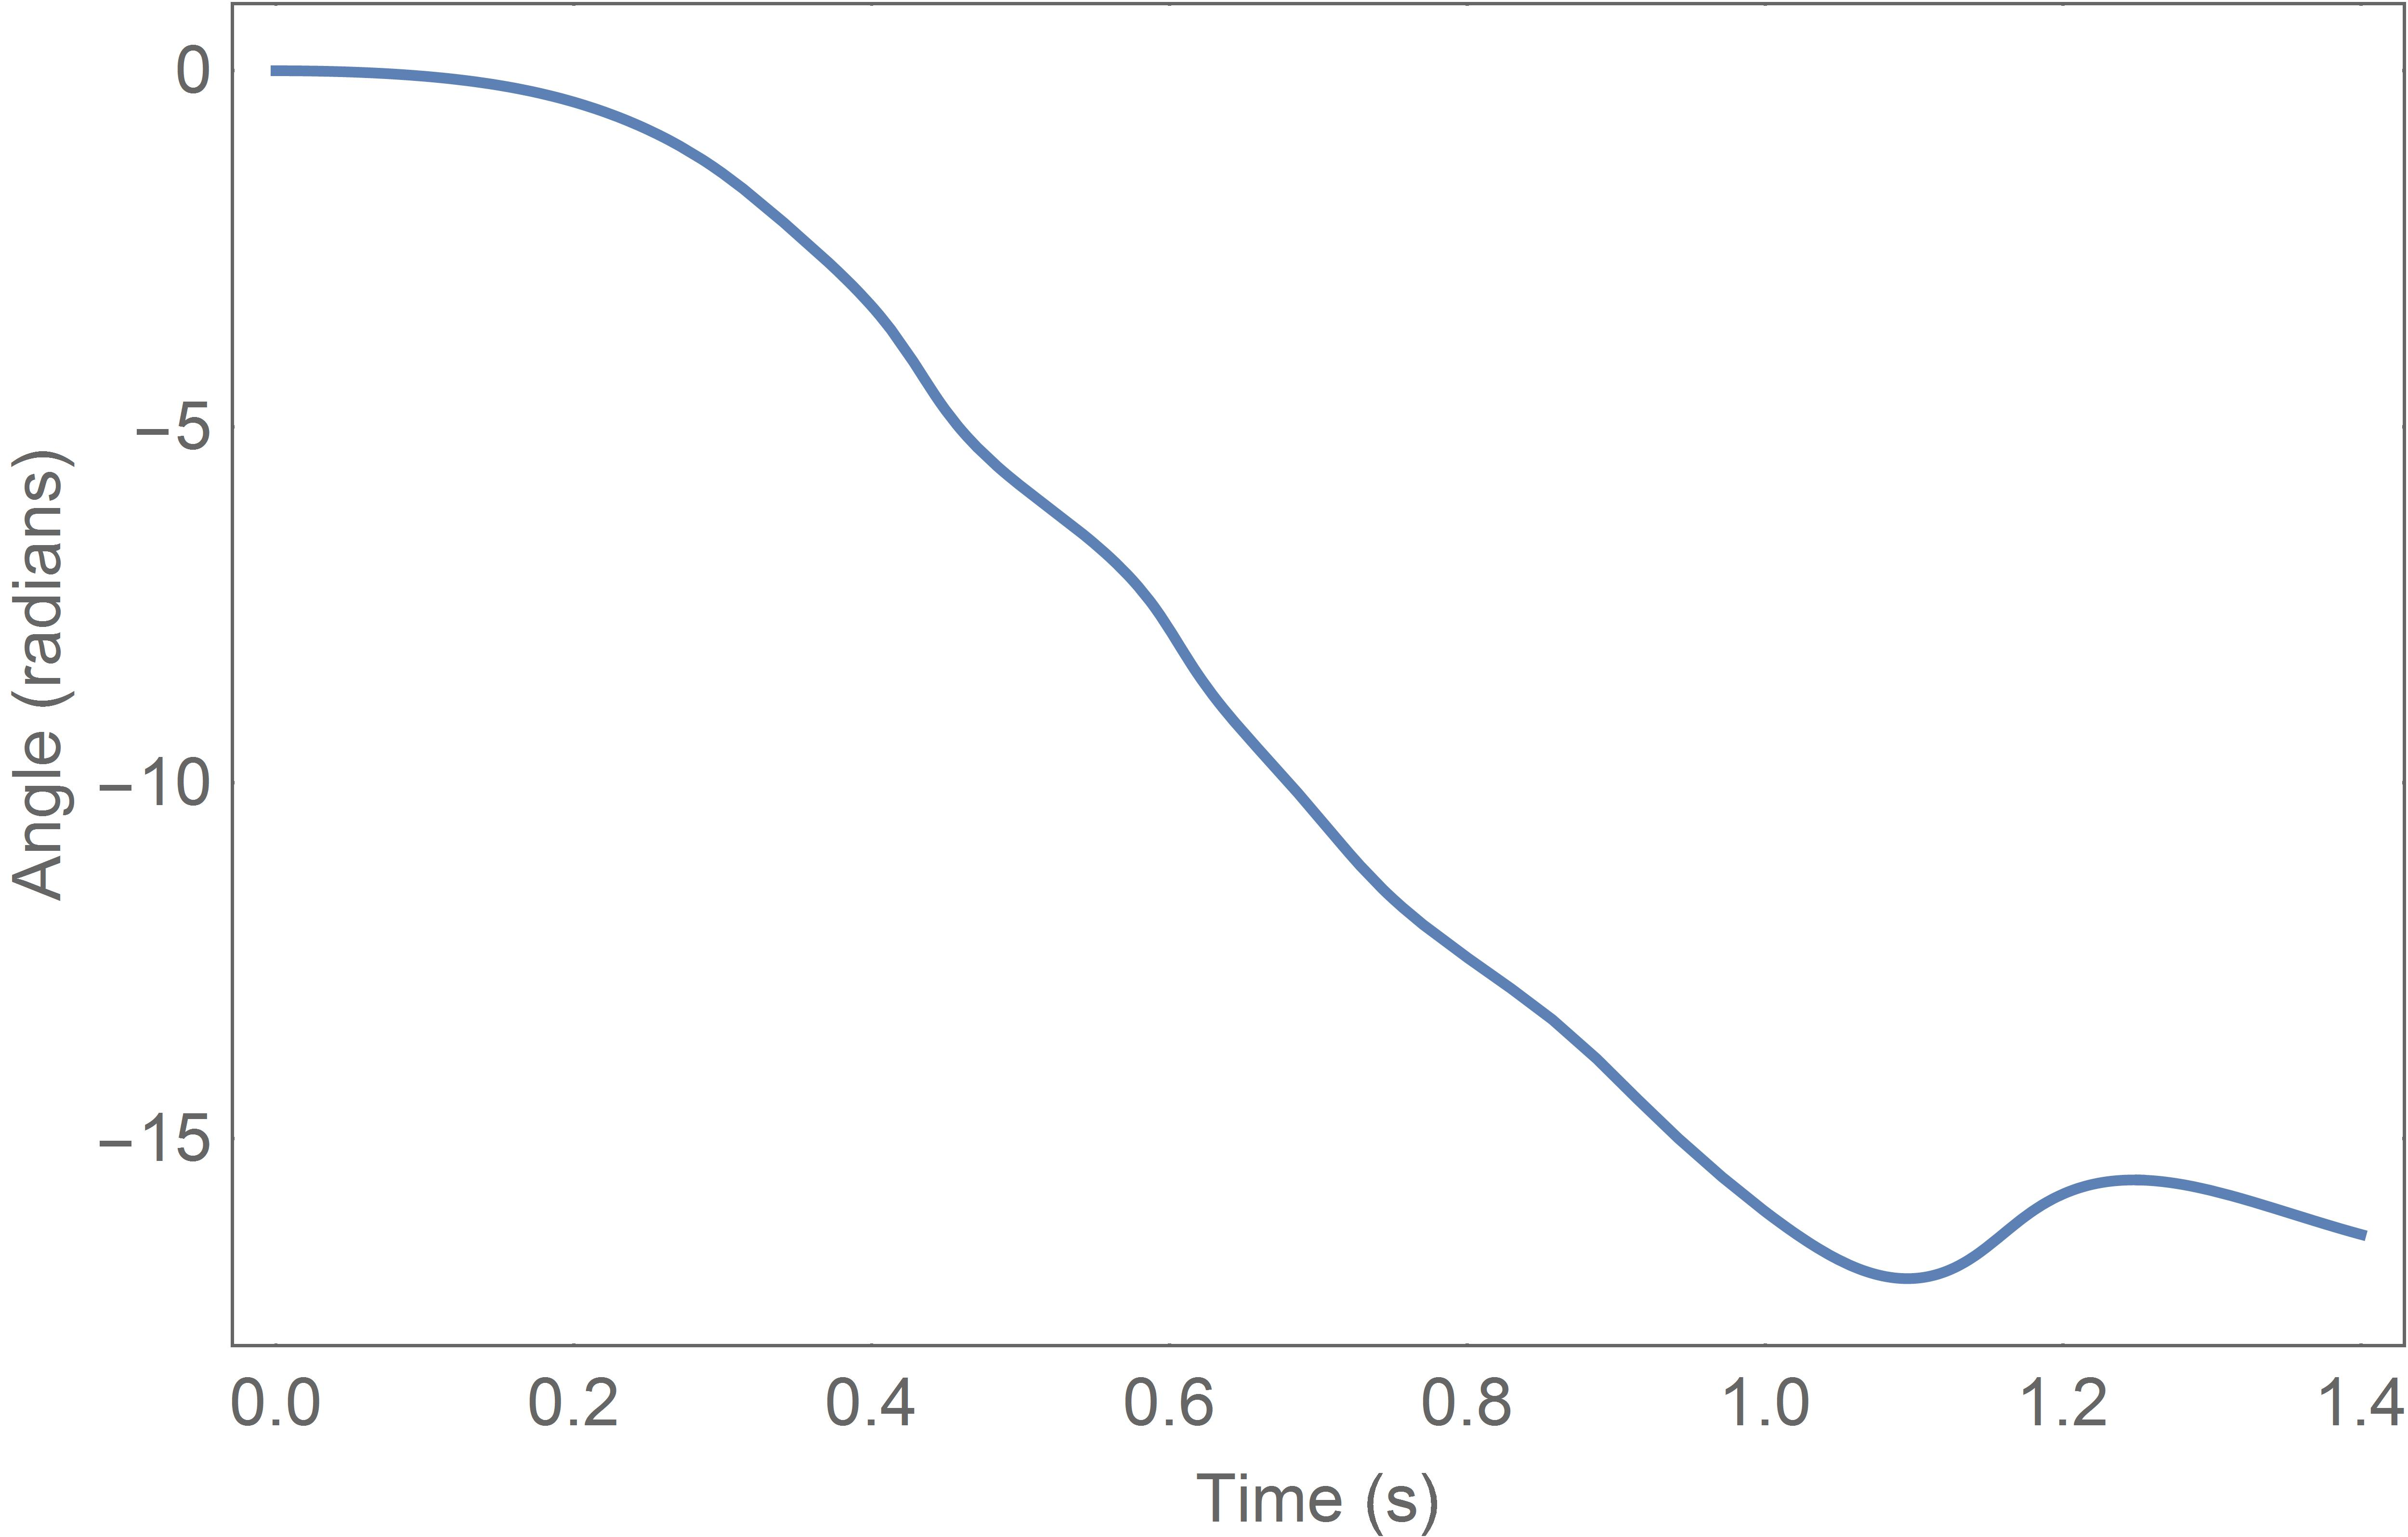
\includegraphics[width=\linewidth]{fallthetafc}
	\endminipage\hspace{1em}%
	\minipage{0.4\textwidth}
	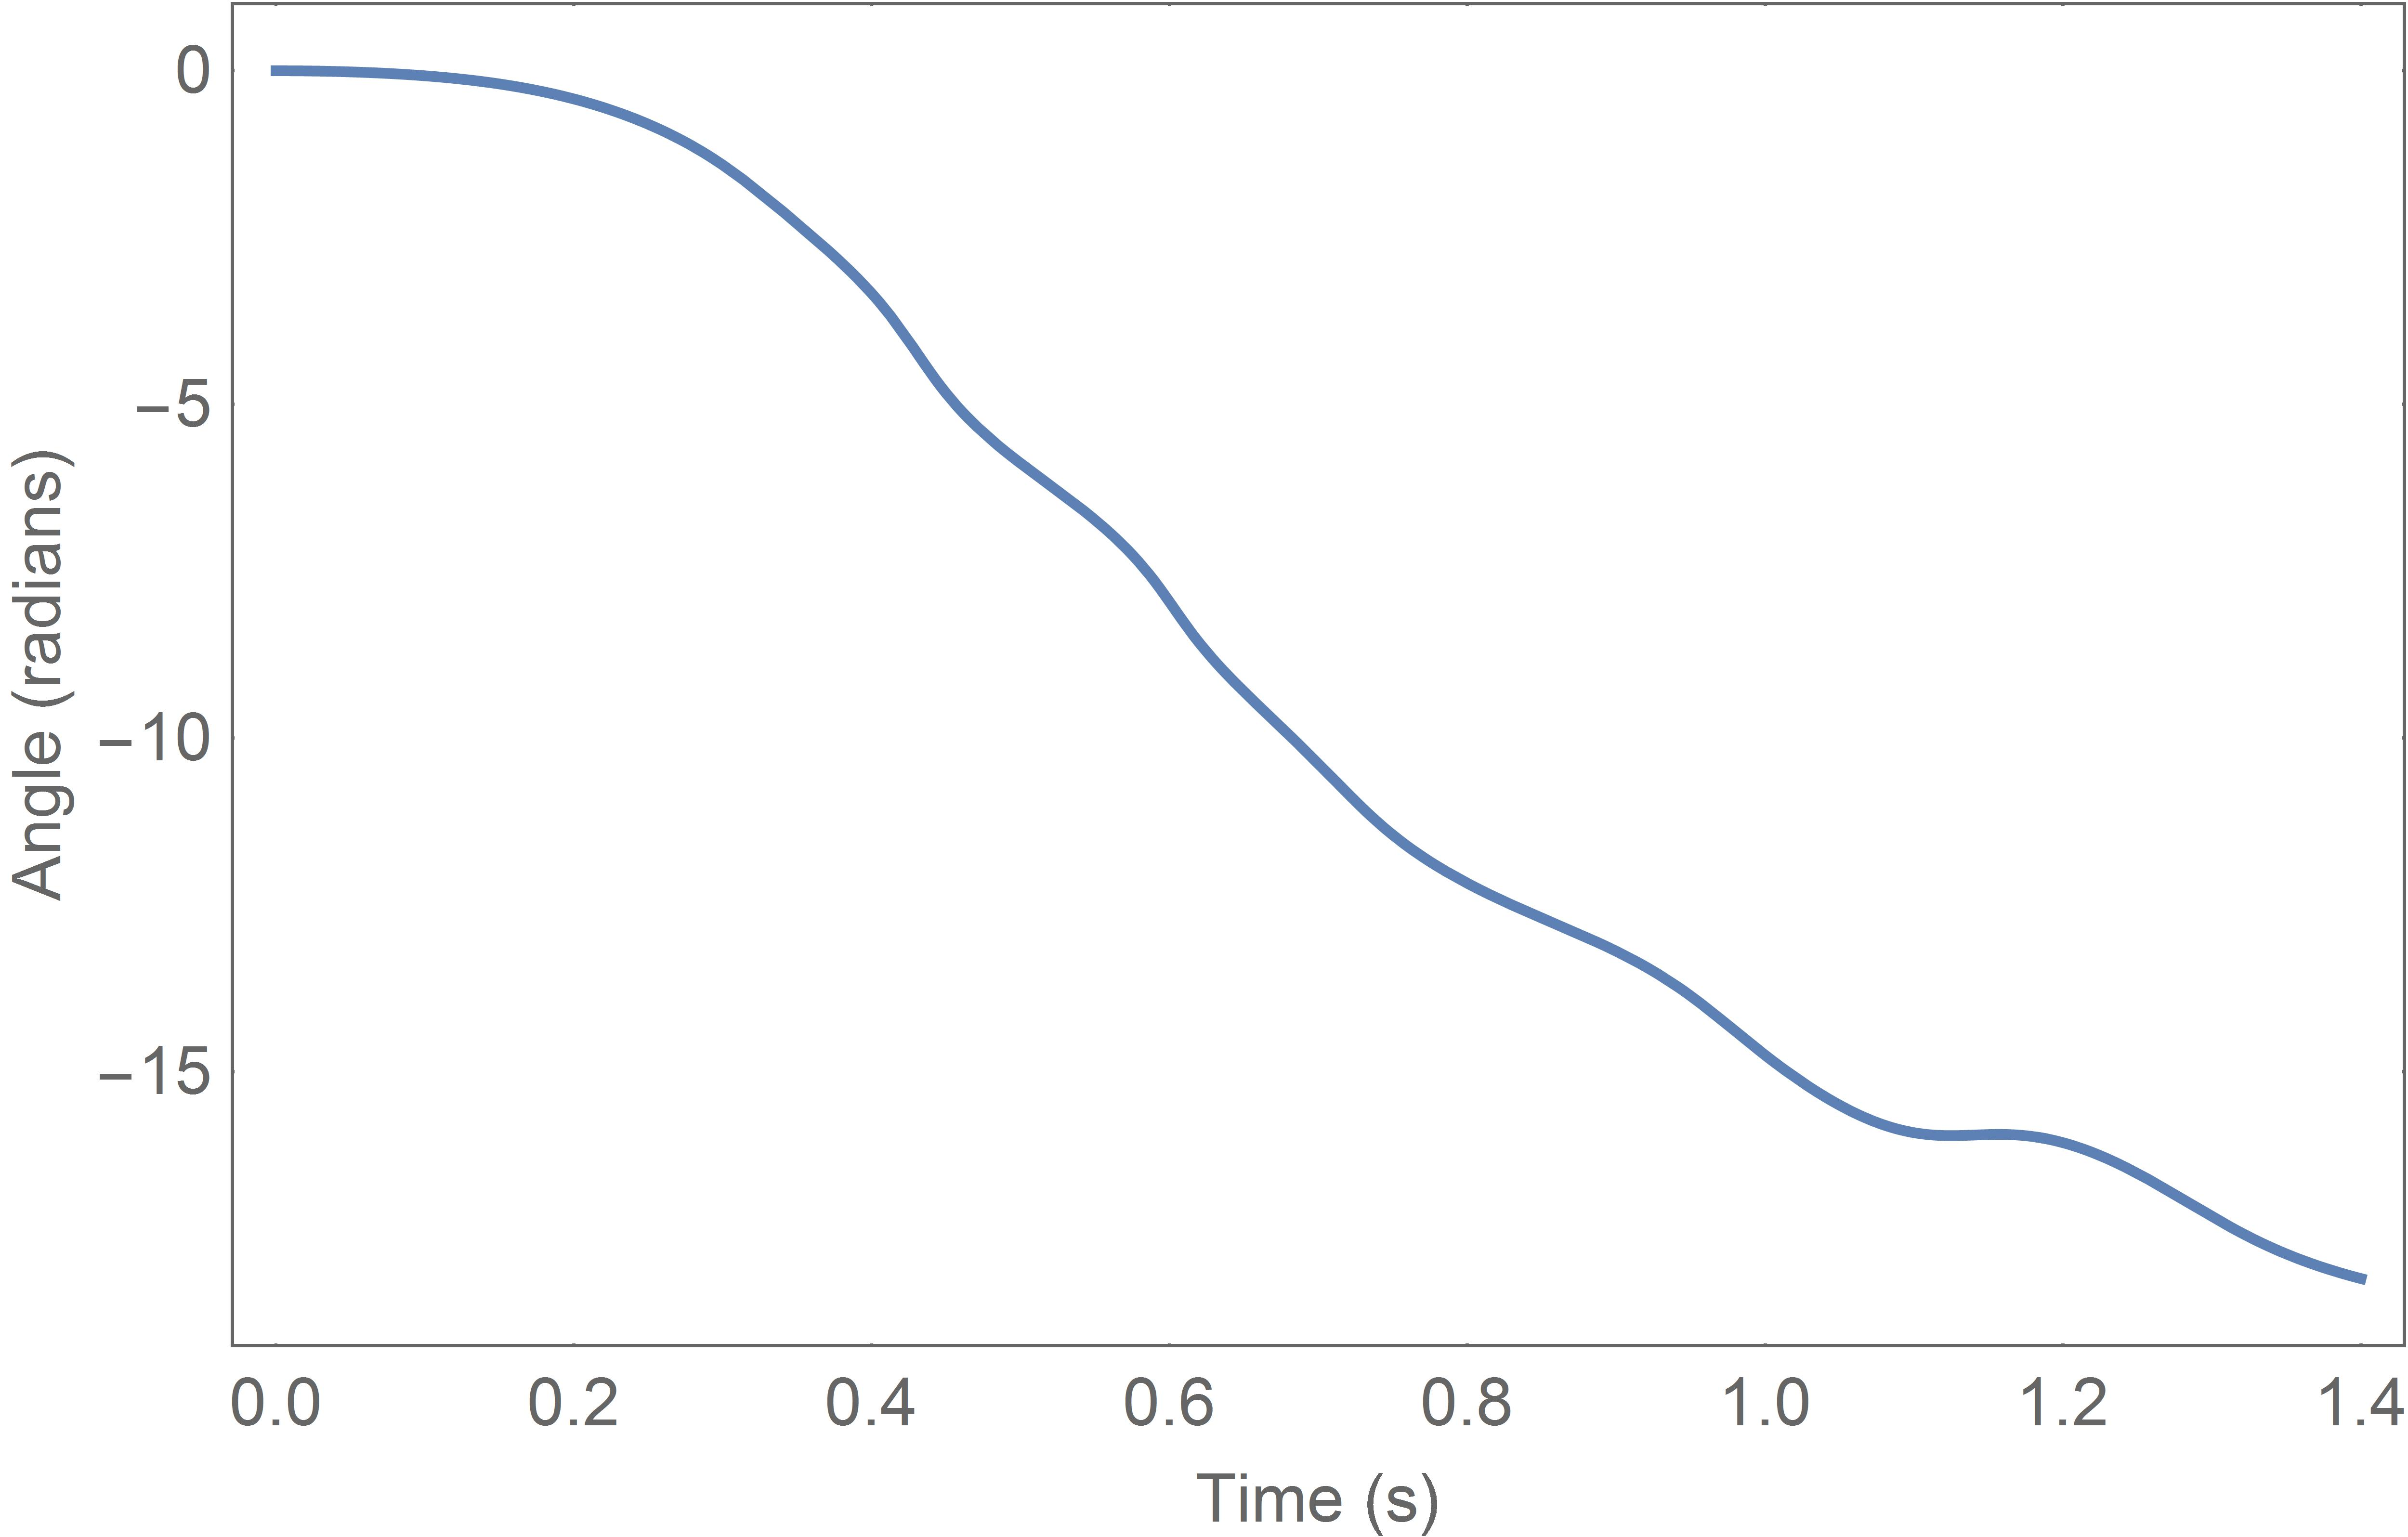
\includegraphics[width=\linewidth]{fallthetabc}
	\endminipage
	\caption{Roll of front caster ($\theta_{fc}$) and back caster ($\theta_{bc}$) as the RipStik falls}\label{fig:fallcaster}	
\end{figure}

The $z$-position plot in Figure \ref{fig:fallglobal} shows the Ripstik falling through the ground plane and reorienting itself in the upright position. 
This is clearly illustrated by the oscillations shown in the first plot.


The roll of the front plate ($\alpha_{fp}$) and back plate ($\alpha_{bp}$) plots in Figure \ref{fig:fallplates} show the plates rotating nearly one full revolution, then rotating fully back to their orgin. 
This clearly describes the behaviour as the RipStik flips through the ground plane.
The yaw of the front caster ($\theta_{fc}$) and back caster ($\theta_{bc}$) plots in figure \ref{fig:fallcaster} describe the motion of the casters as the RipStik falls.
The casters pivot to follow the falling motion of the RipStik and satisfy the nonholonomic constraints.
\par
An accurate visualization can be produced to model the motion of the RipStik. The initial upright and final fallen over position of the RipStik are shown in Figure \ref{fig:fallcaster}

\begin{figure}[!htb]
	\centering
	\minipage{0.4\textwidth}
	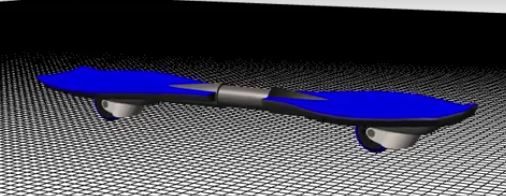
\includegraphics[width=\linewidth]{rest}
	\endminipage\hspace{1em}%
	\minipage{0.37\textwidth}
	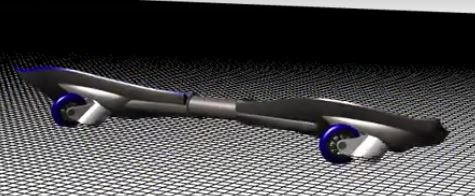
\includegraphics[width=\linewidth]{fall}
	\endminipage
	\caption{Initial upright and final fallen over positions of the RipStik}\label{fig:fallcaster}	
\end{figure}

\subsection{Linear Quadratic Regulator Control}
For the RipStik system, LQR control is intended to be used to stabilize the RipStik about the unstable equilibrium point in its upright position. 
This means keeping the RipStik platforms stable and level, with the control system forces designed to return the RipStik to this configuration under the effect of external perturbations (i.e. rider instability).

The first concern when implementing LQR control is the effect of the nonholonomic constraints on the linearization process. 
In attempting to solve for the Lagrange multipliers in the linearized equations of motion, two potential methods are considered:
\begin{itemize}
	\item Linearize the system with the unknown constraints to produce a linear DAE then solve for the Lagrange Multipliers
	\item Solve for the Lagrange multipliers then linearize the result
\end{itemize}
In his Master's thesis \textit{Linearization and Stability of Nonholonomic Mechanical Systems} \cite{LinNonHolo}, S.D Yang demonstrated a sufficient condition for the commutation of linearizing the equations of motion and solving for Lagrange multipliers. 
In particular, these operations commute at critical points of the potential function \cite{LinNonHolo}.
The test case developed for LQR control consisted of a rolling wheel (as shown in section \ref{sec:testcaserw}) with an inverted pendulum attached (similar to what was shown in \ref{sec:testcaseip}). 
Since both components of the mechanical system have been previously developed and validated, minimal additional work is needed to develop the combined system. 

\subsubsection{Test Case - Rolling Wheel with Inverted Pendulum}

The system and associated dimensions are shown in Figure \ref{fig:invert}.

\begin{figure}[!htb]
	\centering
	\minipage{0.5\textwidth}
	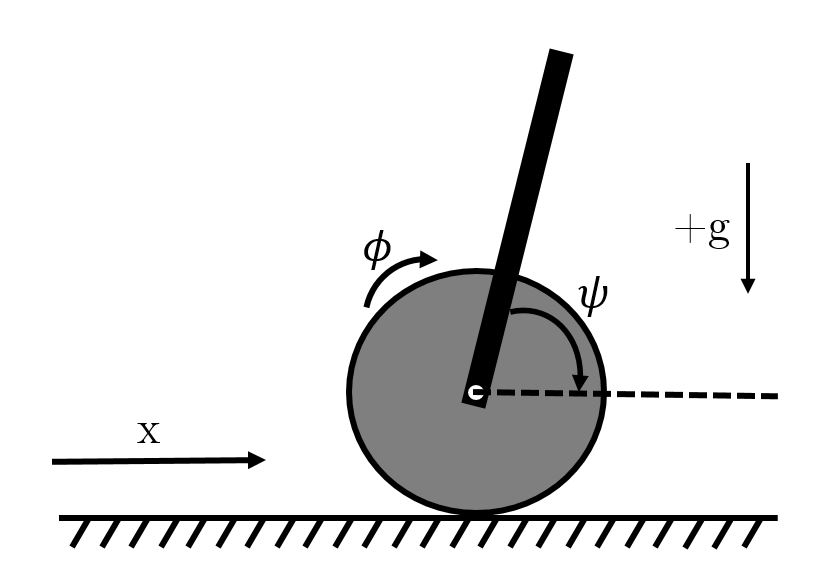
\includegraphics[width=\linewidth]{rollingwheelinvertedpendulum.JPG}
	\caption{The roll angle ($\phi$) and pendulum angle ($\psi$) for the rolling wheel with an inverted pendulum}\label{fig:invert}
	\endminipage
\end{figure}

The two dimensional system has 3 degrees of freedom: the horizontal position $x$, the roll angle $\phi$, and the pendulum angle $\psi$. 
Additionally, the following constants were defined: $m$, the mass of the wheel, $m_p$, the mass of the pendulum, $g$, the acceleration due to gravity, $\rho$, the radius of the wheel, and $L$, the length of the pendulum. 
Note that the pendulum was again modelled as a thin uniform rod.
The moment of inertia of the wheel was defined to be:
\begin{equation}
I_w =
	\begin{pmatrix}
		J_{spin} & 0 & 0 \\
		0 & J_{spin} & 0 \\
		0 & 0 & J_{roll}
	\end{pmatrix},
\end{equation}
Which is consistent with the inertias in Section \ref{sec:testcaserw}. The rod then has a moment of inertia of \textbf{DO WE NEED A SOURCE ON THIS??}
\begin{equation}
I_p =
	\begin{pmatrix}
		\frac{1}{3}L^{2}m_p & 0 & 0 \\
		0 & \frac{1}{3}L^{2}m_p & 0 \\
		0 & 0 & 0
	\end{pmatrix}.
\end{equation}
The unconstrained Lagrangian of the system was computed to be: 
\begin{equation}
\underbrace{m_P \left( g L \sin (\psi (t))- 
	g \rho + 
	\frac{2}{3}L^2 \psi '(t)^2 - 
	L \psi '(t) \sin (\psi (t)) x'(t)+
	\frac{1}{2} x'(t)^2\right)}_{\text{pendulum}} +
	\underbrace{\frac{1}{2} \left(J_{spin} \phi '(t)^2 + 
	m x'(t)^2\right)}_{\text{wheel}} = 0.
\end{equation}
Applying the Euler-Lagrange equation, the unconstrained equations of motion for the system were computed to be: 
\begin{equation}
L m_{P} \psi ''(t) \sin (\psi (t))+L m_{P} \psi
   '(t)^2 \cos (\psi (t))-(m+m_{P}) X''(t)=0
\end{equation}
\begin{equation}
   -J_{spin} \phi''(t)=0
\end{equation}
\begin{equation}
   \frac{1}{3} L m_{P} \left(3 g \cos (\psi (t))-4 L \psi ''(t)+3 \sin (\psi (t)) X''(t)\right)=0
\end{equation}
Additionally, the system has one nonholonomic constraint, expressed as:
\begin{equation}
x'(t) = \rho\theta'(t).
\end{equation}
A control input $u(t)$ was then added to the second equation of motion, thereby applying a torque to the roll angle of the wheel.

In order to experimentally validate the presented result on commutation of linearization and solving for nonholonomic constraints, both procedures were applied to the system. 
They both produced the constrained linear system:
\begin{equation}
	\frac{\left(4 J_{spin}+\rho ^2 (4 m+m_{P})\right)
   \left(L m_{P} \psi ''(t)+(m+m_{P}) X''(t)\right)-\rho 
   u(t) (4 m+m_{P})}{4 J_{spin}+\rho ^2 (4
   m+m_{P})}=0
\end{equation}
\begin{equation}
	\frac{J_{spin} \left(\phi ''(t) \left(4
   J_{spin}+\rho ^2 (4 m+m_{P})\right)-4 u(t)\right)}{4
   J_{spin}+\rho ^2 (4 m+m_{P})}=0
\end{equation}
\begin{equation}
	L m_{P} \left(4 L
   \psi ''(t)+3 X''(t)\right)=0,
\end{equation}
This demonstrates that the result applies as expected for this small system. 
The linearized control system about the unstable equilibrium $\{x=0,\psi=-\frac{\pi}{2},\phi=0\}$ is given by the equation:
\begin{equation}
\left(
\begin{array}{c}
 x'(t) \\
 x''(t) \\
 \psi'(t) \\
 \psi''(t) \\
 \phi'(t) \\
 \phi''(t) \\
\end{array}
\right)
=
\left[
\begin{array}{cccccc}
 0 & 1 & 0 & 0 & 0 & 0 \\
 0 & 0 & -\frac{3 g m_{P} \rho ^2}{4 J_{spin}+\rho ^2 (4
   m+m_{P})} & 0 & 0 & 0 \\
 0 & 0 & 0 & 1 & 0 & 0 \\
 0 & 0 & \frac{3 g \left(J_{spin}+\rho ^2
   (m+m_{P})\right)}{L \left(4 J_{spin}+\rho ^2 (4
   m+m_{P})\right)} & 0 & 0 & 0 \\
 0 & 0 & 0 & 0 & 0 & 1 \\
 0 & 0 & -\frac{3 g m_{P} \rho }{4 J_{spin}+\rho ^2 (4
   m+m_{P})} & 0 & 0 & 0 \\
\end{array}
\right]
\left(
\begin{array}{c}
 x(t) \\
 x'(t) \\
 \psi(t) \\
 \psi'(t) \\
 \phi(t) \\
 \phi'(t) \\
\end{array}
\right)
+
\left[
\begin{array}{c}
 0 \\
 \frac{4 \rho }{4 J_{spin}+\rho ^2 (4 m+m_{P})} \\
 0 \\
 -\frac{3 \rho }{L \left(4 J_{spin}+\rho ^2 (4
   m+m_{P})\right)} \\
 0 \\
 \frac{4}{4 J_{spin}+\rho ^2 (4 m+m_{P})} \\
\end{array}
\right]u(t).
\end{equation}
With the system linearized, a stabilizing controller was developed to keep the pendulum at the upright unstable equilibrium position $\{x=0,\psi=-\frac{\pi}{2},\phi=0\}$. 
To do this, values were chosen for each of the parameters in the system and a state weighting matrix $Q$ was selected based on the project considerations. 
In particular, the aim was to prioritize stability of the pendulum angle $\psi$ and angular velocity of the roll angle $\phi$ since this keeps the operator upright and avoids using large angular accelerations to maintain this stability. 
Meanwhile, it allows the position of the wheel to return more slowly to the equilibrium since the horizontal position of the wheel is not a priority in the stabilization problem for personal electric transport vehicles.

The perturbation function $22 e^{-10 (t-8)^2}-22 e^{-10 (t-12)^2}$ was applied to the roll angle, simulating uneven ground conditions when riding the PET device. 
This applies perturbations of $+22$ and $-22$ at 8 and 12 seconds respectively. The second perturbation was specifically timed such that the system had not fully recovered from the first, demonstrating stability and robustness of the controlled system.
\par

\begin{figure}[!htb]
	\centering
	\minipage{0.4\textwidth}
	\includegraphics[width=\linewidth]{perturbation.png}
	\endminipage\hspace{1em}%
	\caption{The perturbation function that was applied to the rolling wheel with inverted pendulum plotted as a function of time}\label{fig:perturb}
\end{figure}

\begin{figure}[!htb]
	\centering
	\minipage{0.4\textwidth}
	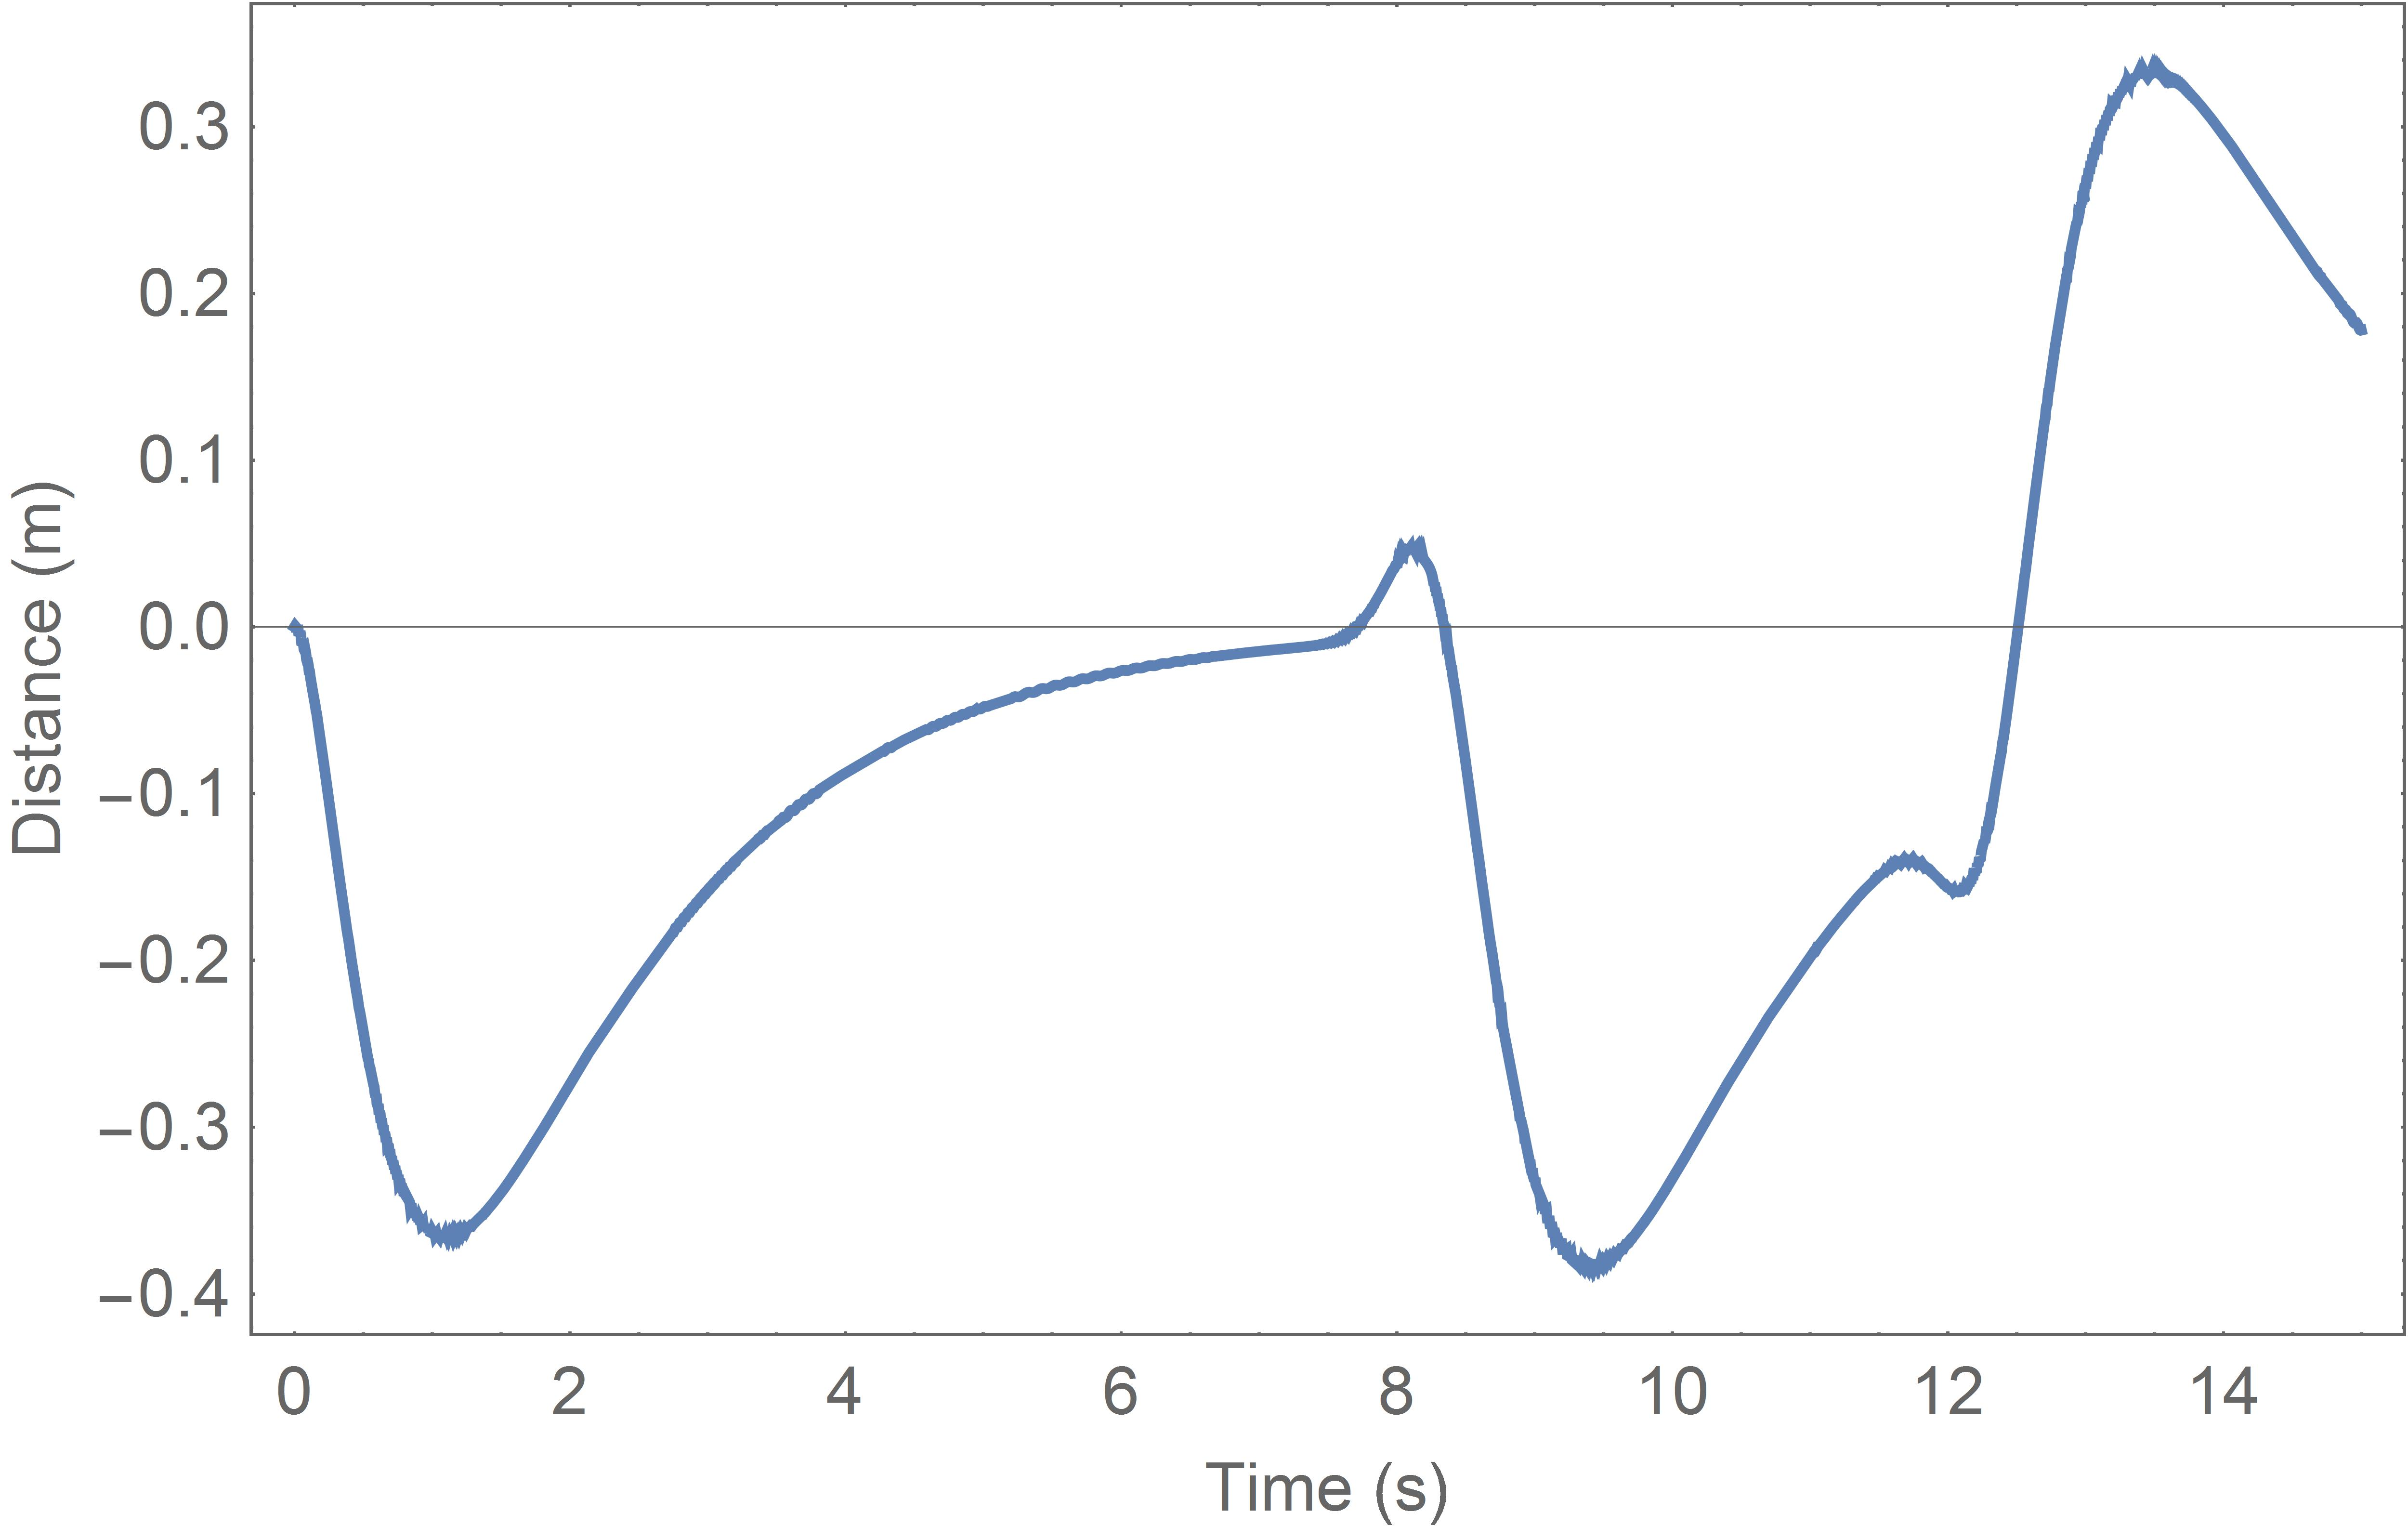
\includegraphics[width=\linewidth]{wheelperturbdistance.jpg}
	\endminipage\hspace{1em}%
	\caption{The X-position of the wheel plotted as a function of time}\label{fig:wheelperturbdistance}
\end{figure}

\begin{figure}[!htb]
	\centering
	\minipage{0.44\textwidth}
	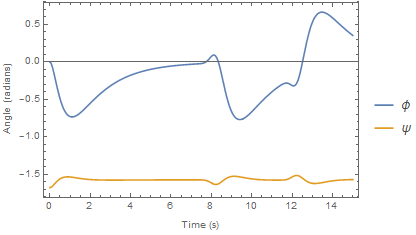
\includegraphics[width=\linewidth]{wheelperturbphipsi.png}
	\endminipage\hspace{1em}%
	\caption{The roll angle ($\phi$) and the pendulum angle ($\psi$) plotted as a function of time}\label{fig:wheelperturbphipsi}
\end{figure}

\par
\subsubsection{Model Implementation Challenges}
Three main challenges must be investigated in extrapolating these LQR results to the larger RipStik system. These are:
\begin{itemize}
	\item Ongoing complexities regarding numeric integration
	\item Uncertainty about the effects of including control forces in the commutation of linearization and solving for Lagrange multipliers
	\item The possible effects of linearization on system behaviour
\end{itemize}
A brief discussion of each follows.
\paragraph{Numeric Integration}\mbox{}\\
Adding control forces may further aggravate the previously discussed issues with system stiffness in the RipStik. 
This would occur if the control forces cause the system to react quickly, creating rapid changes in dynamics that the numeric integrator will not be able to accurately replicate.
\paragraph{Control Forces in Commutation}\mbox{}\\
While the commutation of solving for Lagrange multipliers was demonstrated \cite{LinNonHolo} at points where the potential force is zero, the result may not extend to include the equations of motion with the control forces since they are non-zero. 
While the result was demonstrated with control forces on the rolling wheel with pendulum, it may be due to the simplicity of the system. 
To ensure that this holds on all systems, including the RipStik, a formal proof would be required.
\paragraph{Linearization \& System Behavior}\mbox{}\\
It has previously been demonstrated that for some mechanical systems, linearization will produce an uncontrollable system despite that the nonlinear system may be controllable and that, intuitively, there should exist a control law \cite{CCSMCS}. 
For example, this can arise from decoupling when the initial velocities are zero. 
In the context of the RipStik, the system is sufficiently large that identifying these types of issues would be difficult since it may not be possible to draw conclusions about the local controllability of the nonlinear system.


